\chapter{Elastic Cloud Compute}\label{ch:ec2}

\section{AWS Setup}\label{sec:aws-setup}

After the VPC and subnets were configured, the initial deployment of the web app began with setting up EC2.
This AWS service allows for scalable computing capacity through the use of a virtual computing environment hosted in the
cloud~\parencite{aws2022ec2}.
The web app will be stored on an EC2 instance of Amazon Linux, known as Amazon Machine Image (AMI), which will then be
launched through a docker container stored on the app.

\begin{figure}[!htbp]
    \centering
    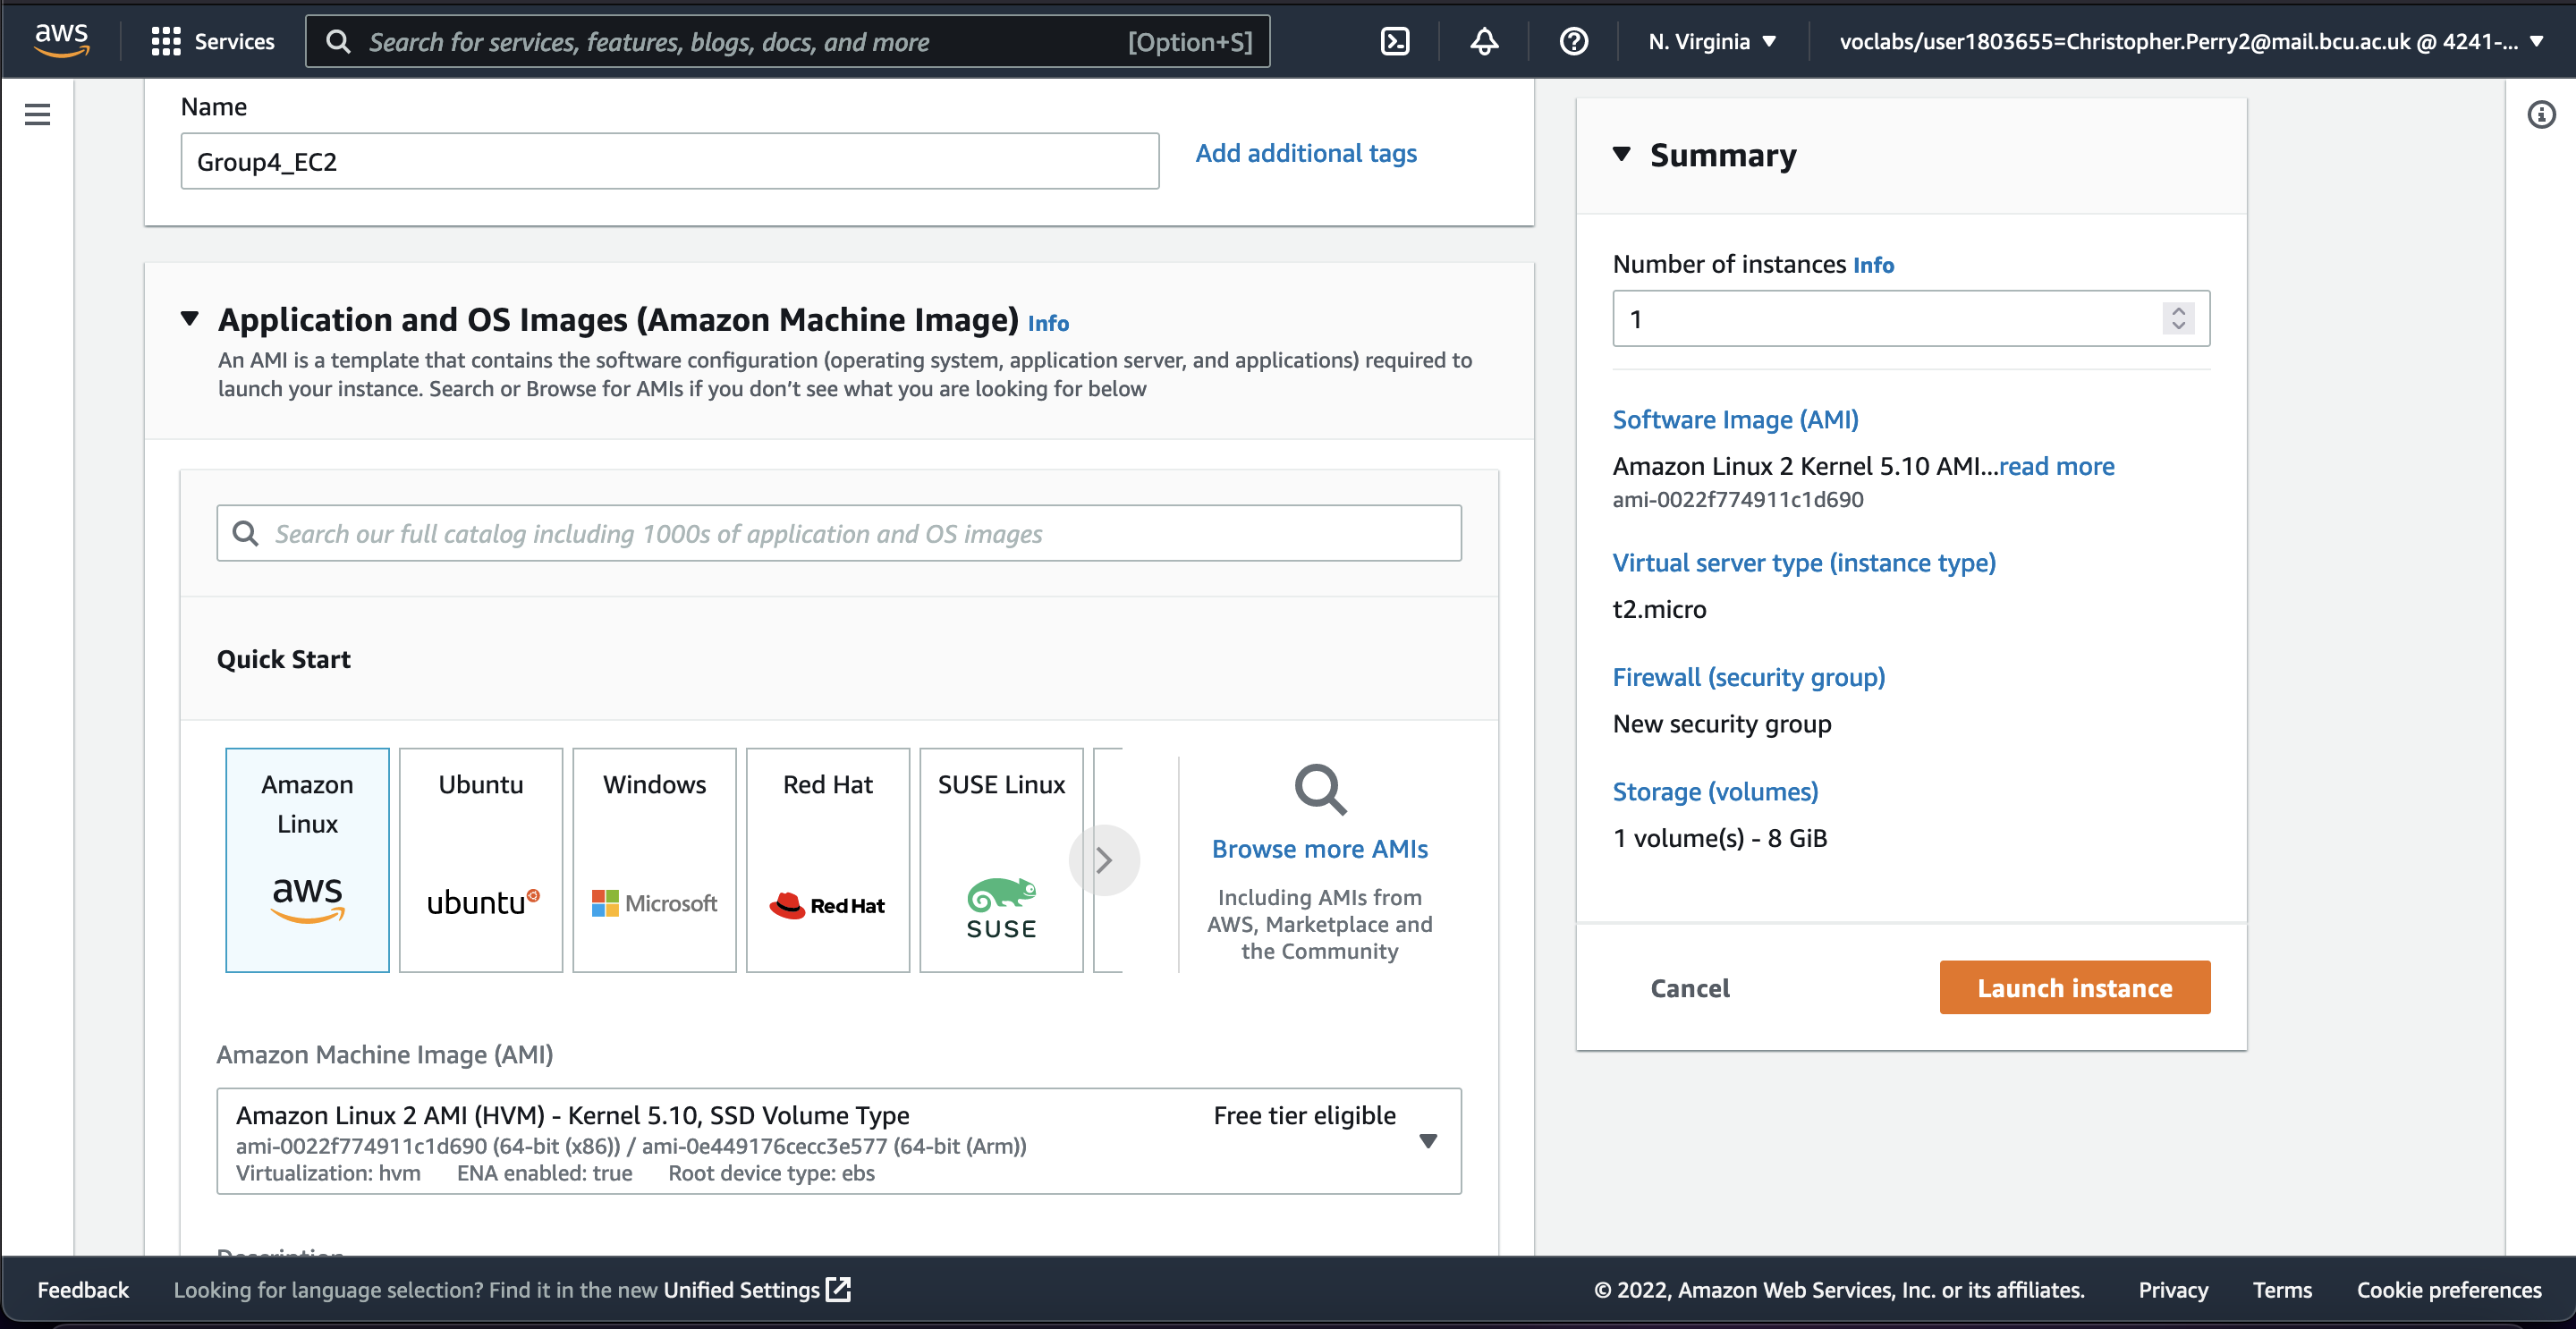
\includegraphics[width=\textwidth]{resources/ec2/create-instance-application-and-os-images}
    \caption{Selection of EC2 OS Image.}
    \label{fig:ec2-os}
\end{figure}

Figure~\ref{fig:ec2-os} details the selection of the Operating System (OS) that will be used for the EC2 instance.
The \textit{Amazon Linux 2} AMI was selected, as it is already configured with Linux and does not need any more setup.

\clearpage
Now that an AMI has been chosen, the specific instance type that will be used within this AMI can be selected.
It was decided that the instance type of \textit{t2.micro} would be used, as it contains only 1GB of Random Access
Memory (RAM).
The selection of this can be found in Figure~\ref{fig:ec2-instance}.

\begin{figure}[!htbp]
    \centering
    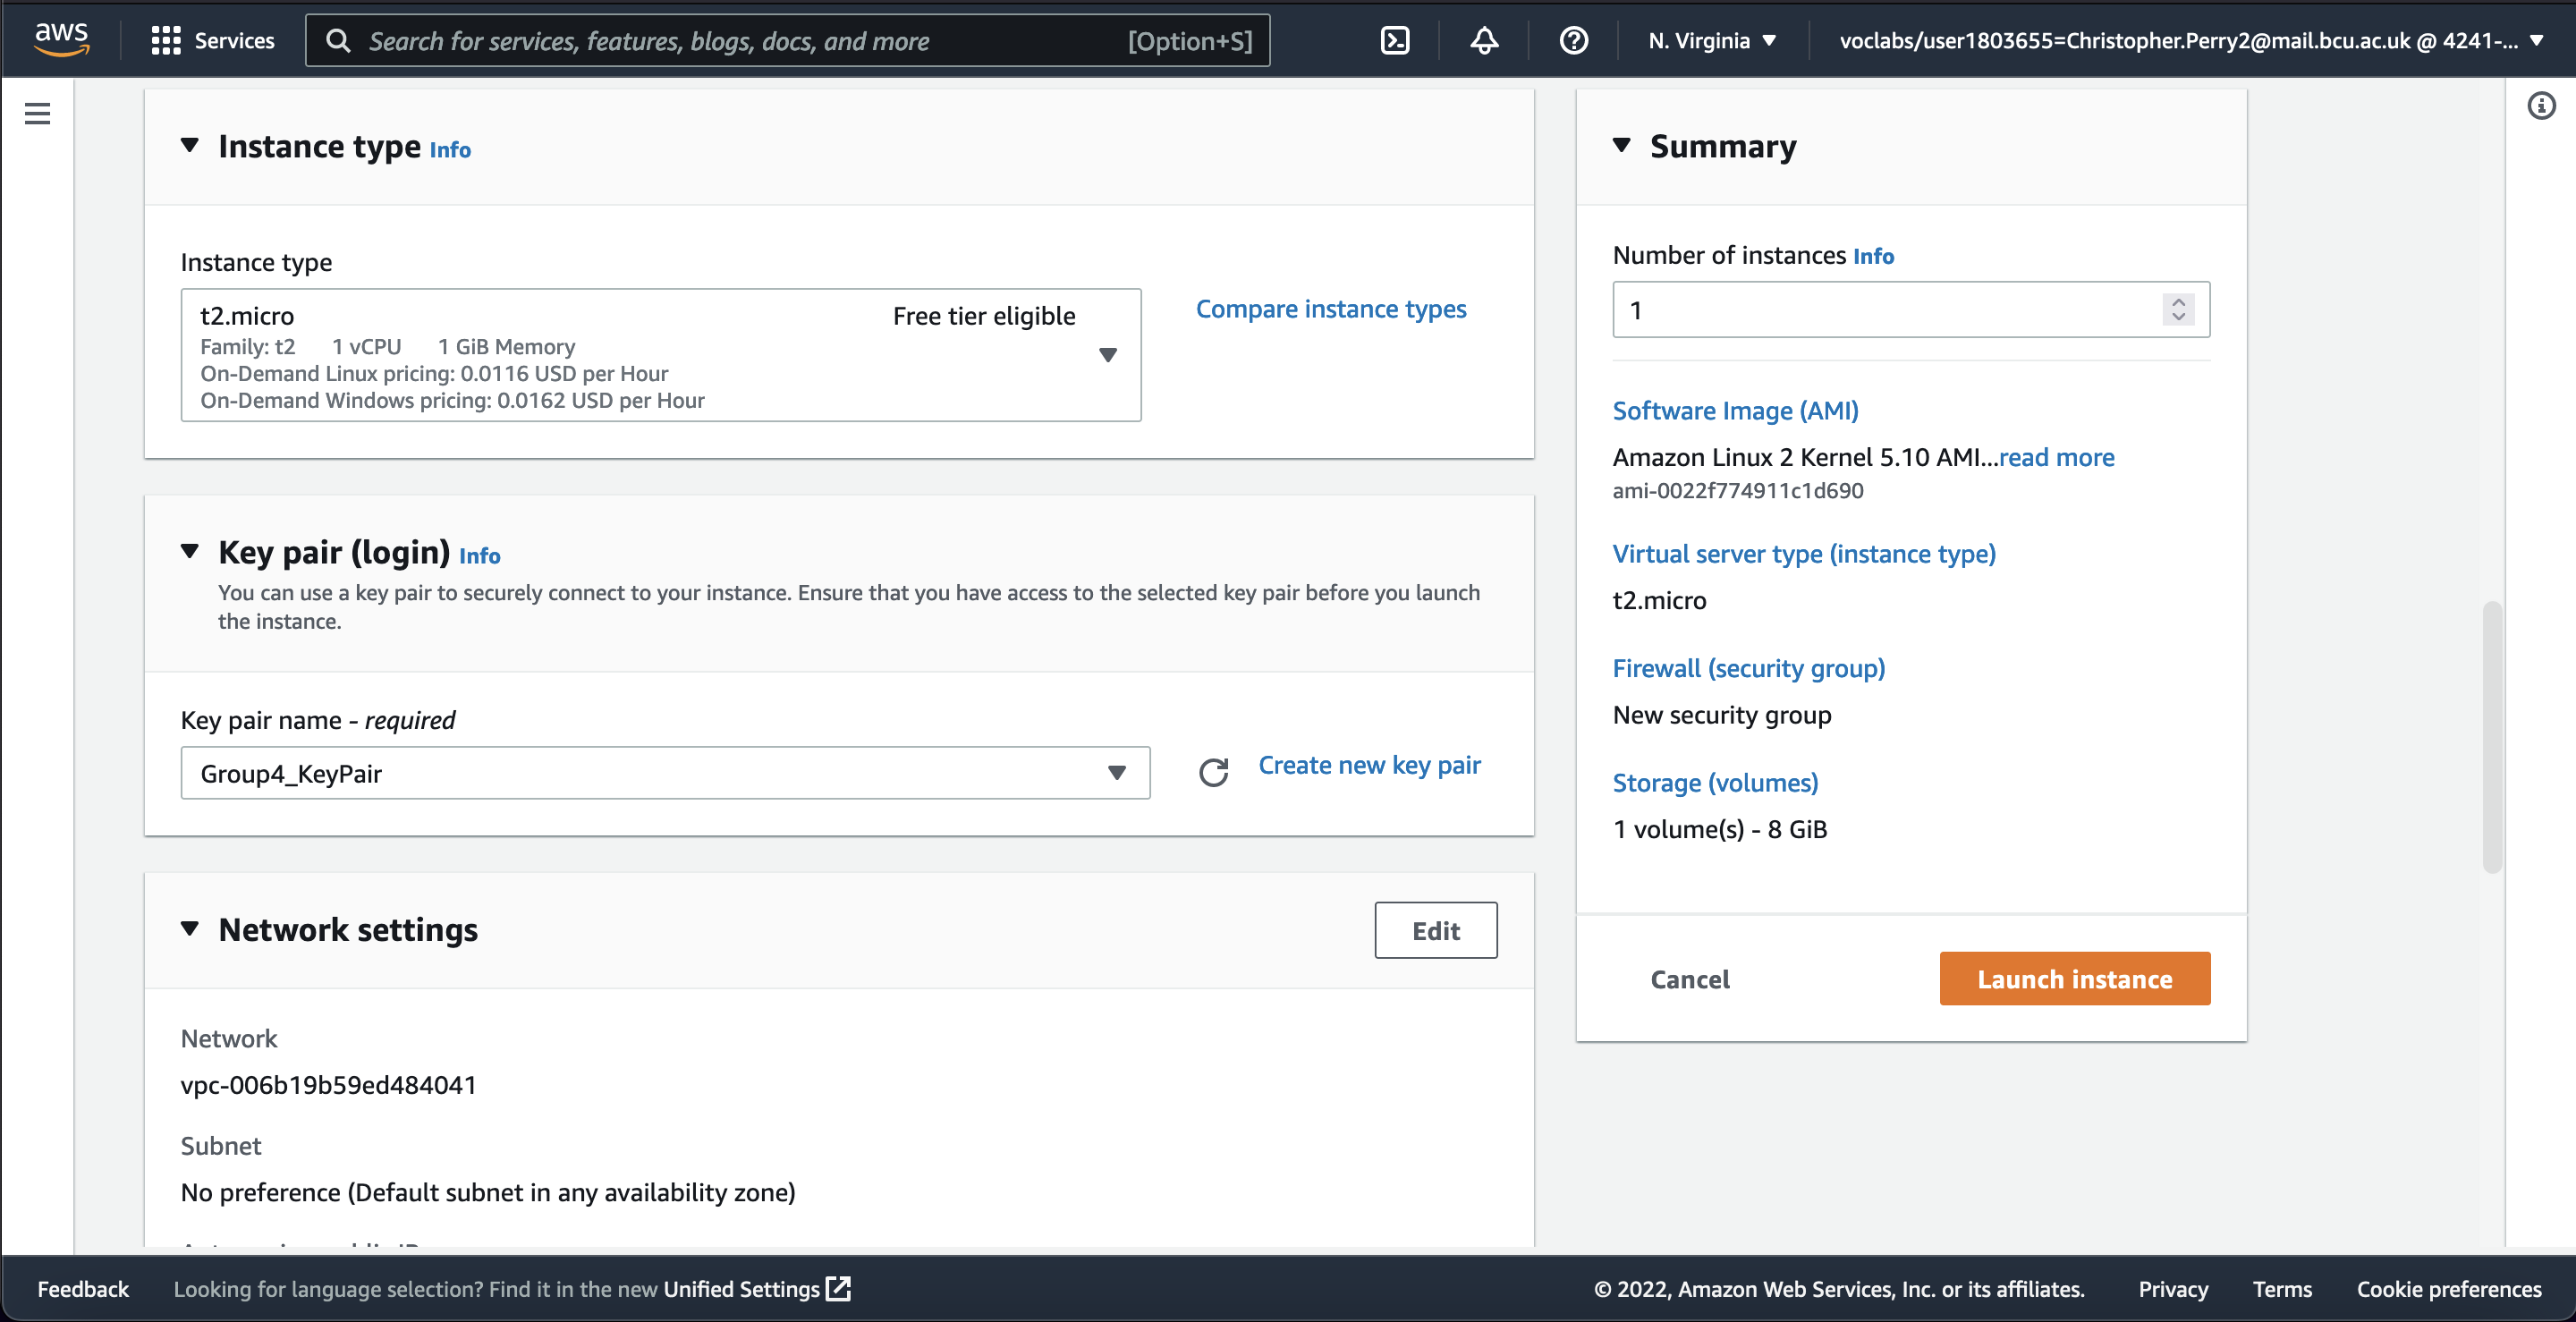
\includegraphics[width=\textwidth]{resources/ec2/create-instance-instance-type}
    \caption{Selection of EC2 Instance.}
    \label{fig:ec2-instance}
\end{figure}

A key pair will allow for the ability to sign in to the EC2 instance with a unique set of login credentials, heightening
the security of the project.

The next stage of the setup process was to set up networking for the EC2 instance, in order for the web app to work with
Docker to download relevant containers from DockerHub, which will allow a Laravel instance to be initialised, as
discussed in Section~\ref{ch:web-app}.

\begin{figure}[!htbp]
    \centering
    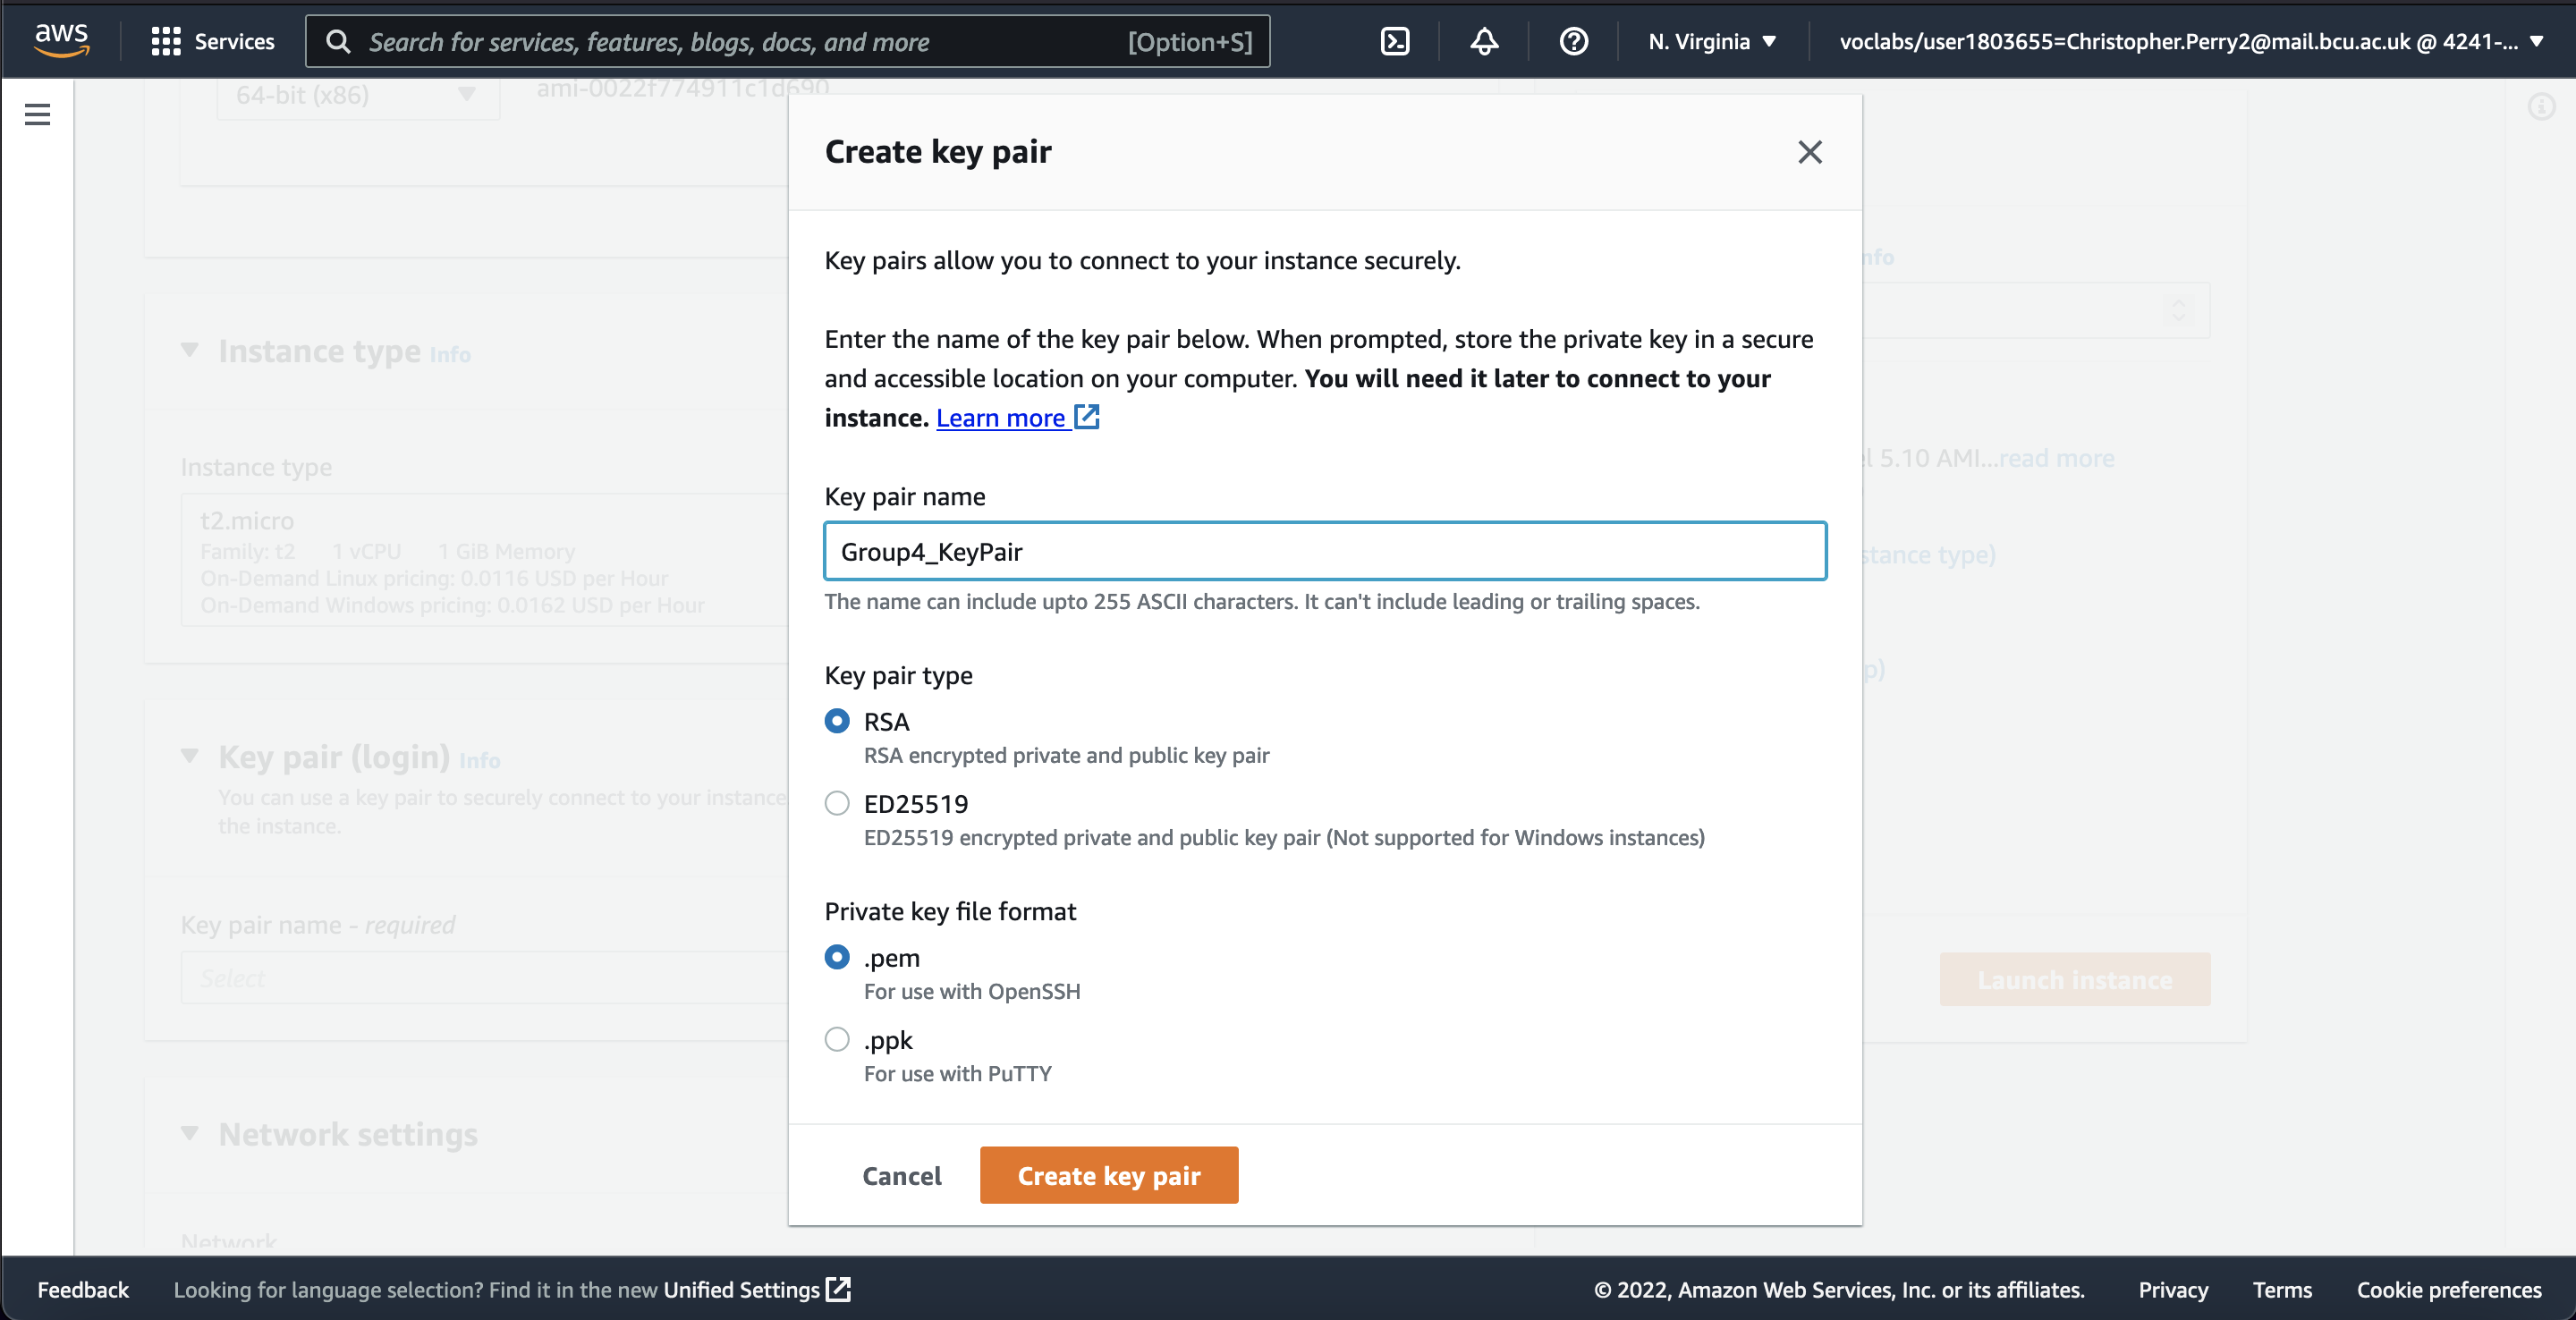
\includegraphics[width=\textwidth]{resources/ec2/create-key-pair}
    \caption{Selection of EC2 Keypair.}
    \label{fig:ec2-keypair}
\end{figure}

This process can be seen in Figure~\ref{fig:ec2-keypair}.

The instance is assigned the VPC created in Section~\ref{ch:vpc-subnets}, where it is assigned a subnet in the same
availability zone of \mintinline{zsh}|us-east-1|.

\begin{figure}[!htbp]
    \centering
    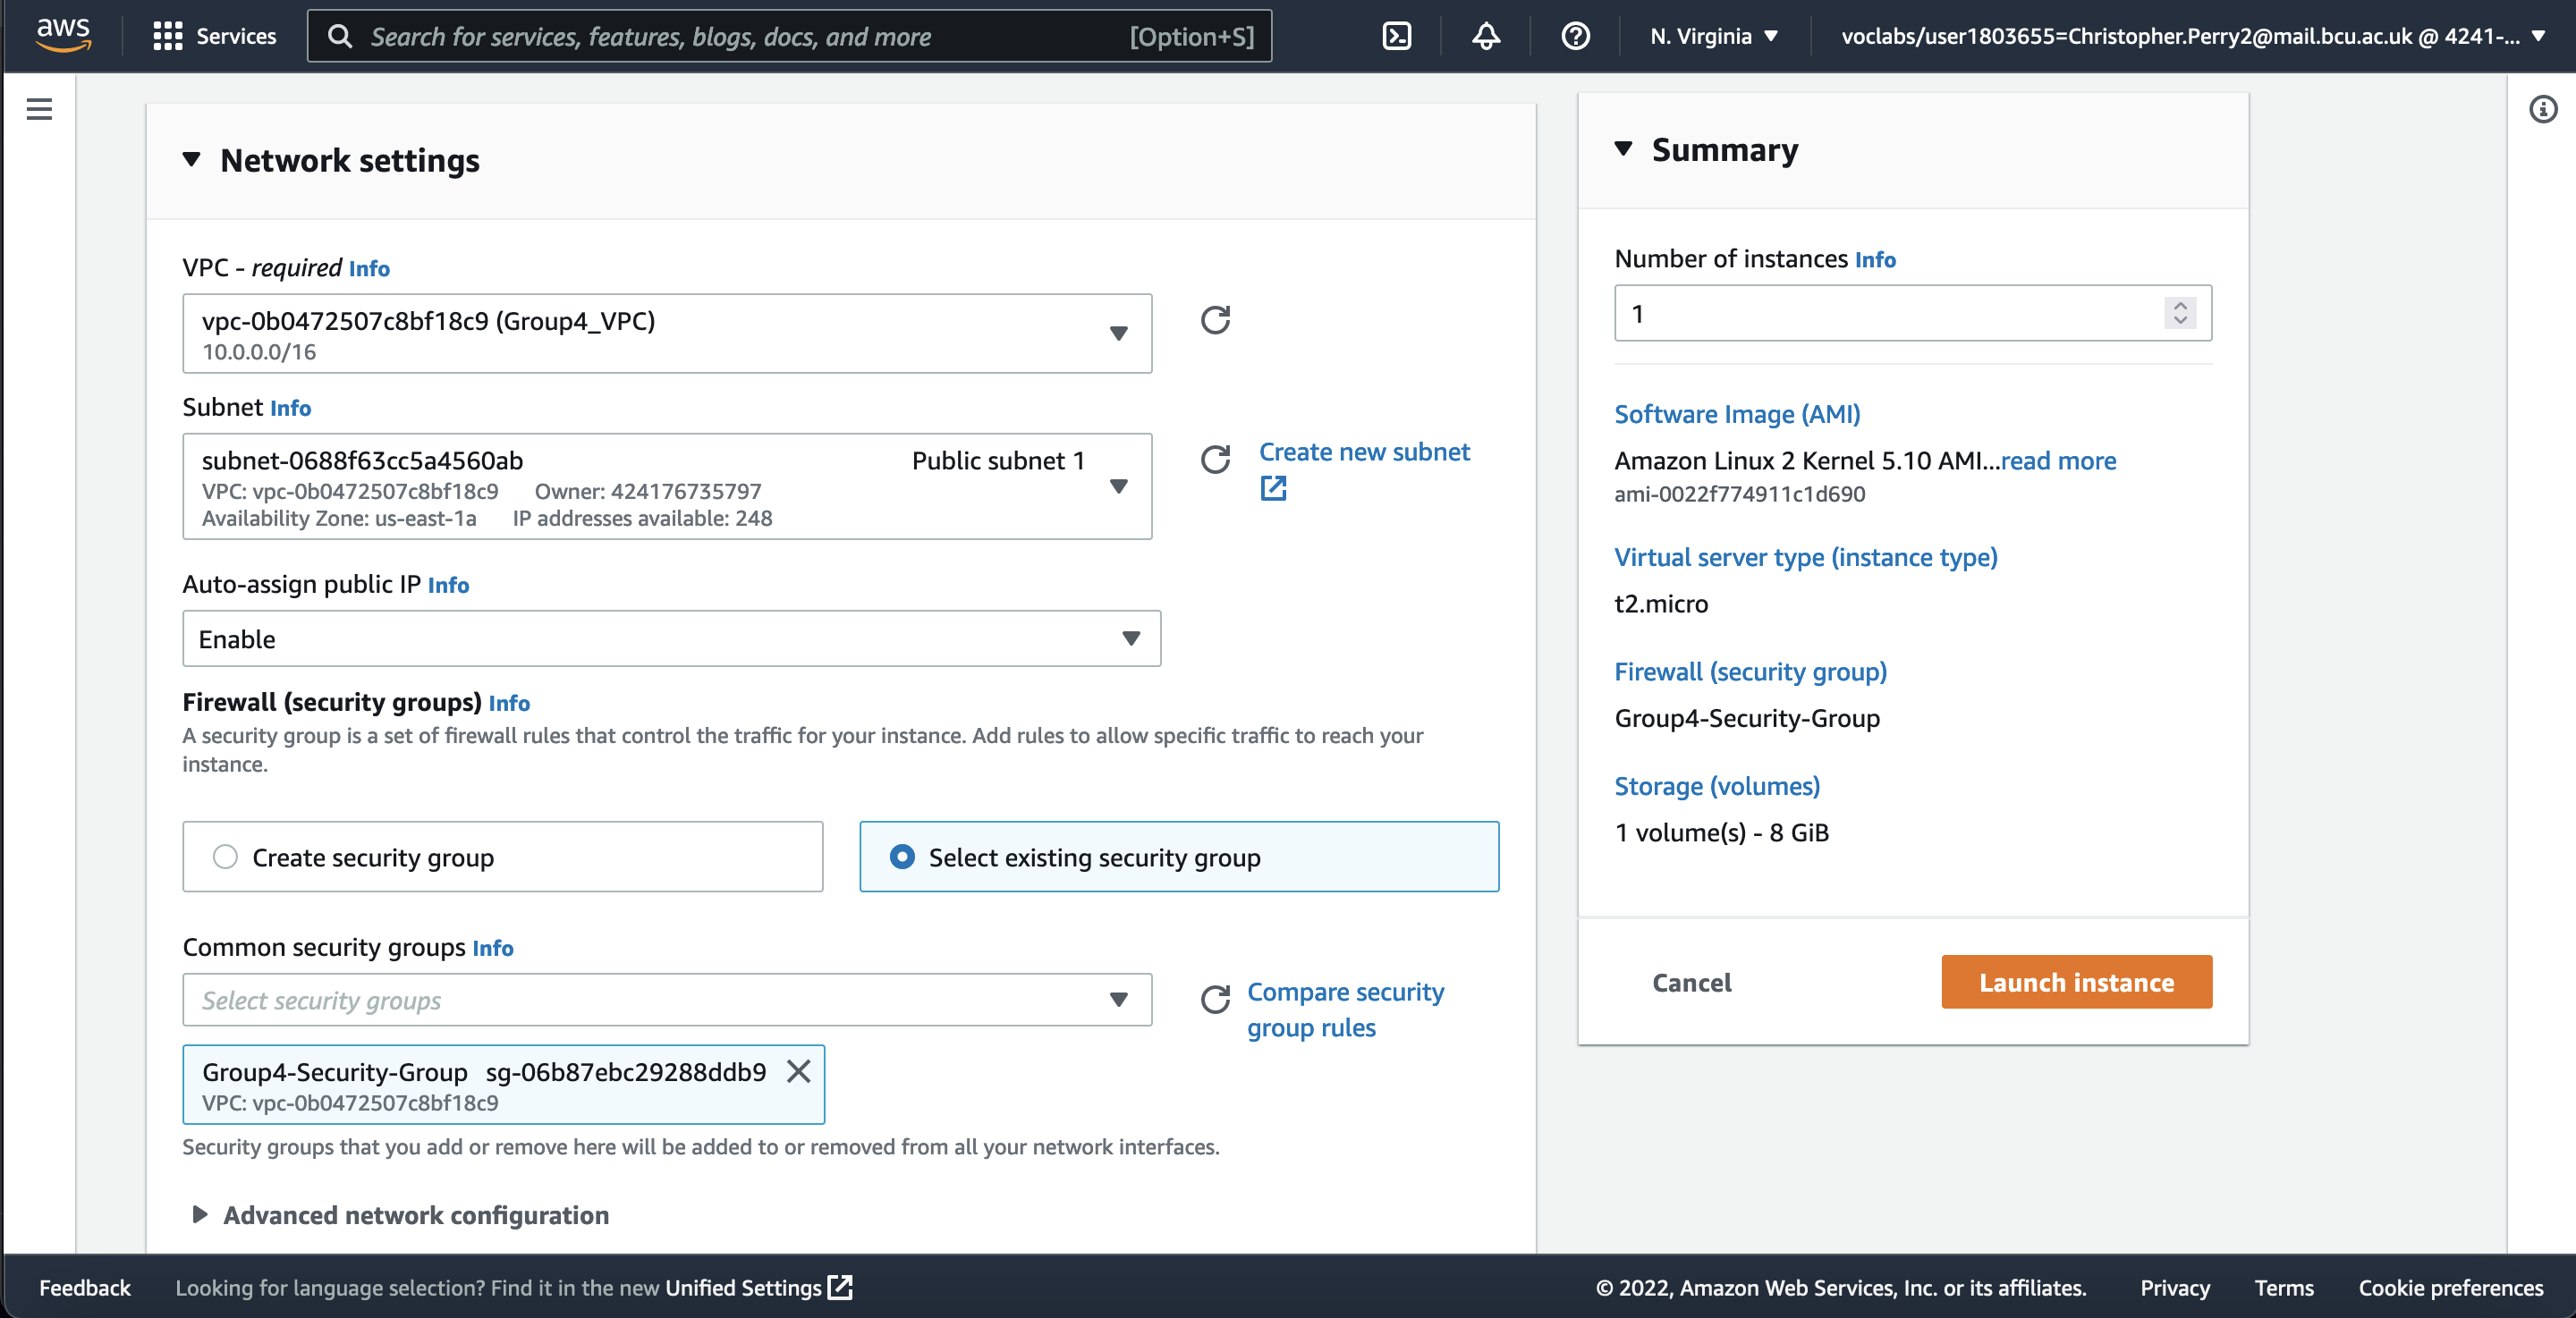
\includegraphics[width=\textwidth]{resources/ec2/create-instance-network-settings}
    \caption{Selection of EC2 Networking options.}
    \label{fig:ec2-networking}
\end{figure}

\begin{figure}[!htbp]
    \centering
    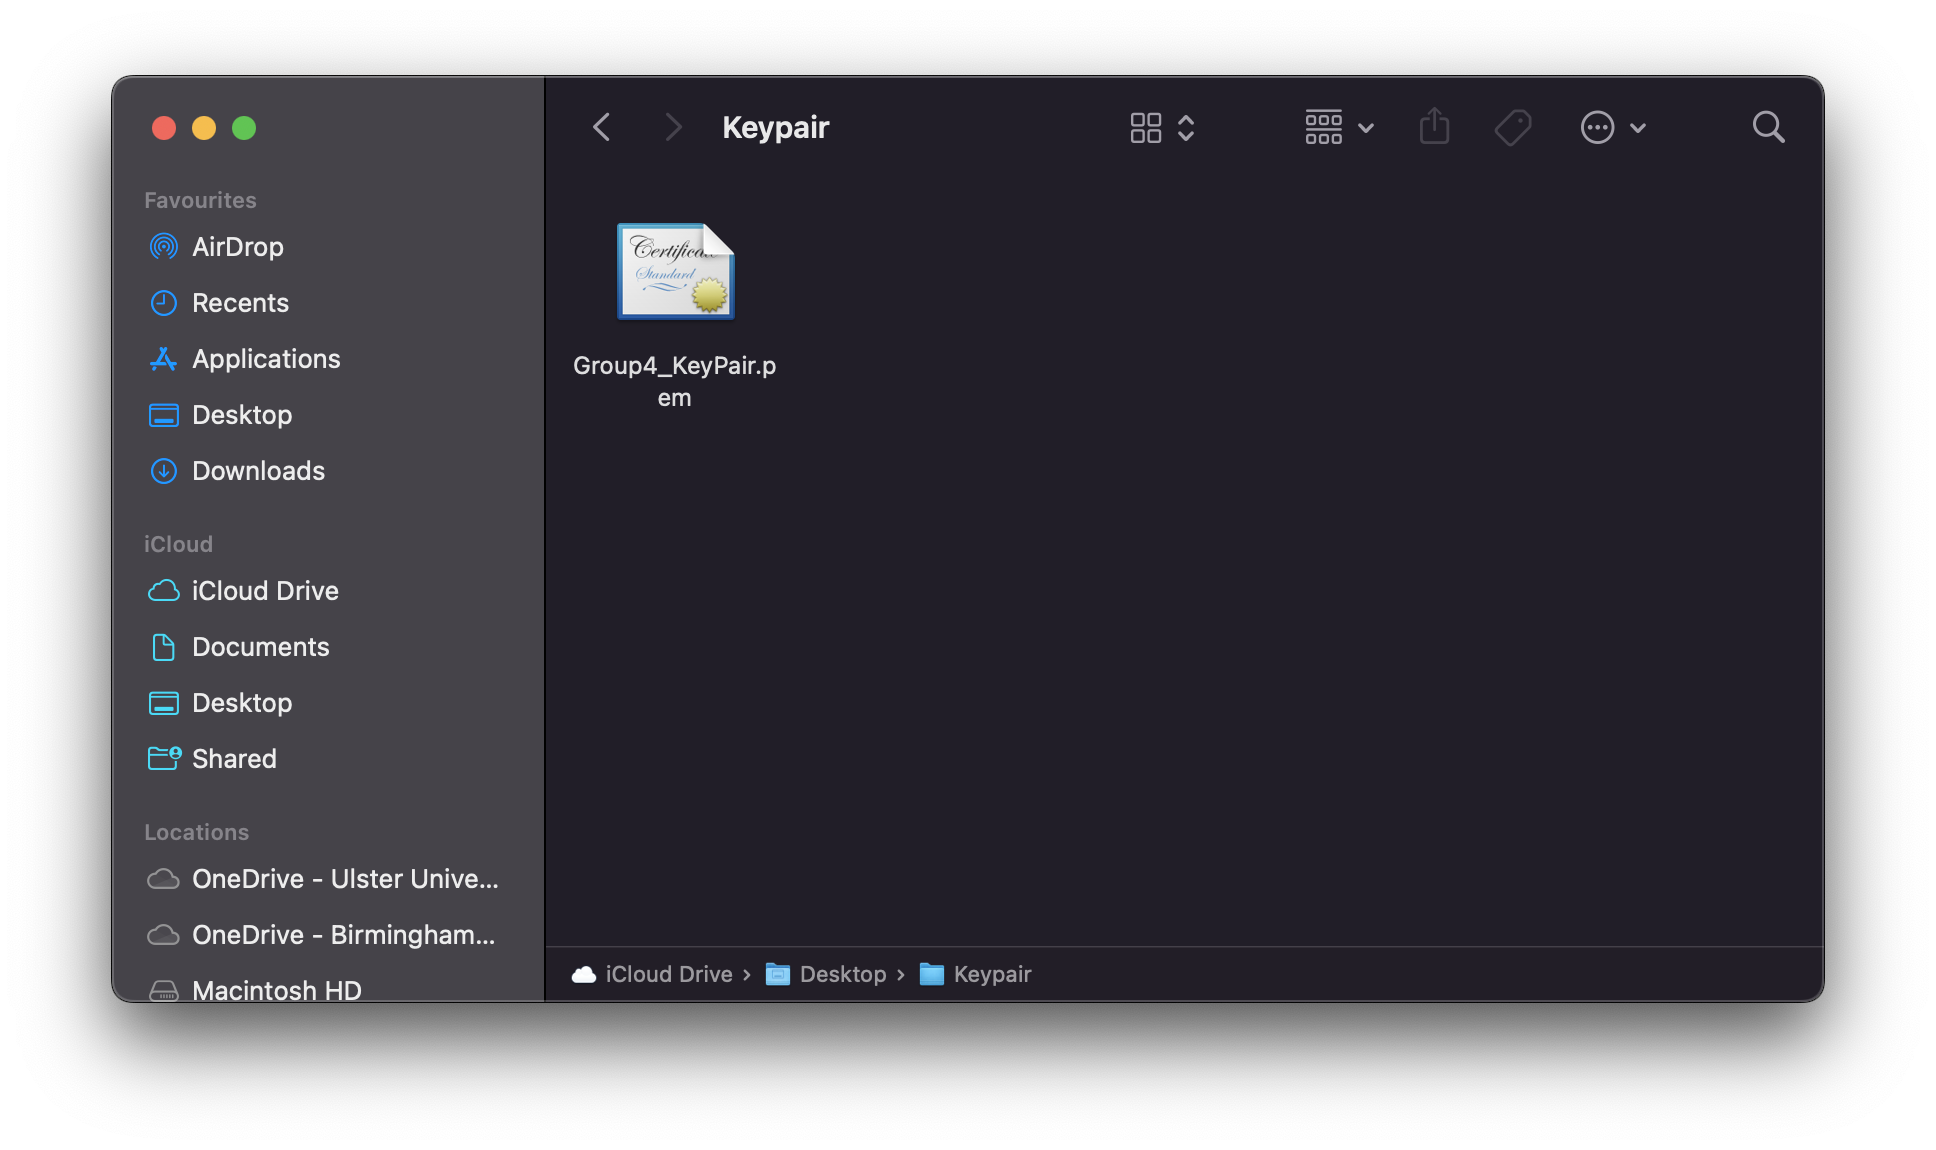
\includegraphics[width=\textwidth]{resources/ec2/keypair}
    \caption{Generated EC2 Keypair in the \mintinline{sql}|.pem| format.}
    \label{fig:keypair}
\end{figure}

This setup can be seen in Figure~\ref{fig:ec2-networking}.
An EC2 keypair is then generated in the \mintinline{sql}|.pem| format.

This is enough to comfortably run the web app without any issues.
Storage for the AMI was subsequently chosen.
It was decided that 8GB of storage would be used, as this is enough to run the web app and still provide leftover
storage for any system-critical tasks.

\begin{figure}[!htbp]
    \centering
    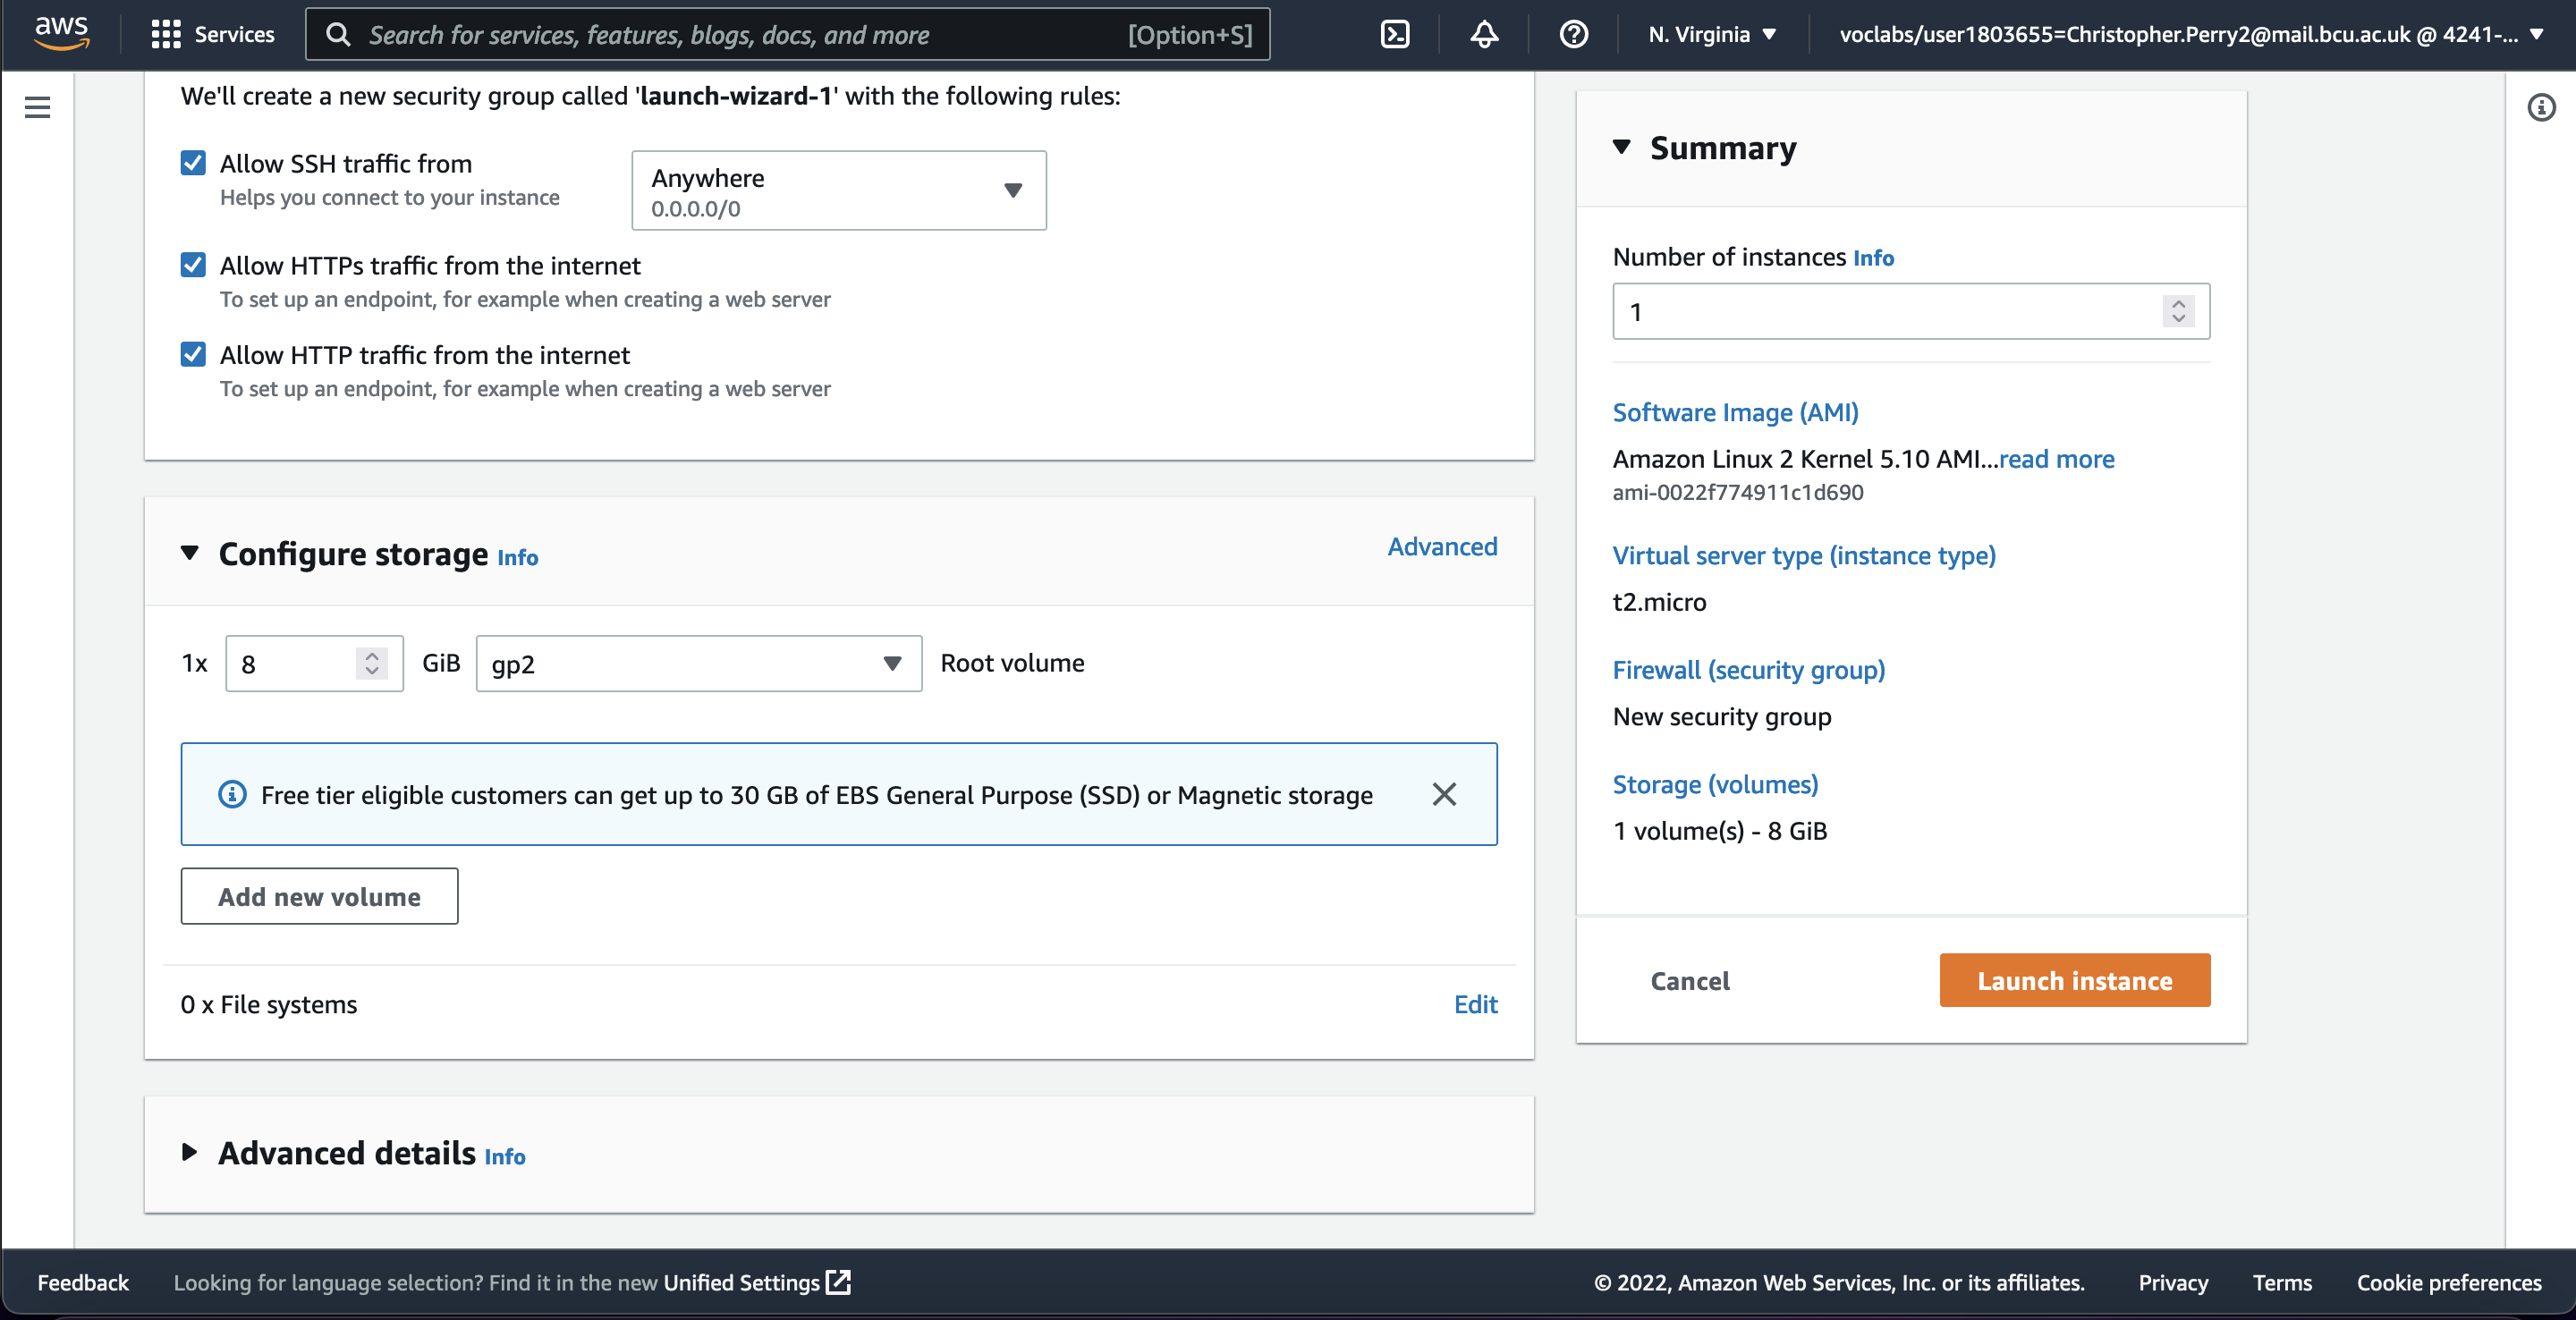
\includegraphics[width=\textwidth]{resources/ec2/create-instance-configure-storage}
    \caption{Selection of EC2 Storage Configuration.}
    \label{fig:ec2-storage}
\end{figure}

The selection of these options can be found in Figure~\ref{fig:ec2-storage}.
In addition to this, the chosen options are eligible for "Free Tier", which means that it will use a limited amount of the
\$100 budget allocated for the project.

\clearpage

\section{EC2 Login}\label{sec:webapp-setup}

The EC2 instance \mintinline{zsh}|group4-ec2| is now live, and the webapp can be loaded onto it.
The instance is first logged in to through the use of the \mintinline{zsh}|ssh| command, followed by the
\mintinline{sql}|-i| argument to specify an identify file, which was generated earlier, and then the public ipv4 address
of the instance.

\begin{figure}[!htbp]
    \centering
    \begin{minted}{zsh}
ssh -i ~/Desktop/Group4_KeyPair.pem ec2-user@52.45.13.111
    \end{minted}
    \caption{SSH command to log into EC2 instance.}\label{fig:ssh-login}
\end{figure}

This command can seen being executed in Figure~\ref{fig:ssh-login}.

\begin{figure}[!htbp]
    \centering
    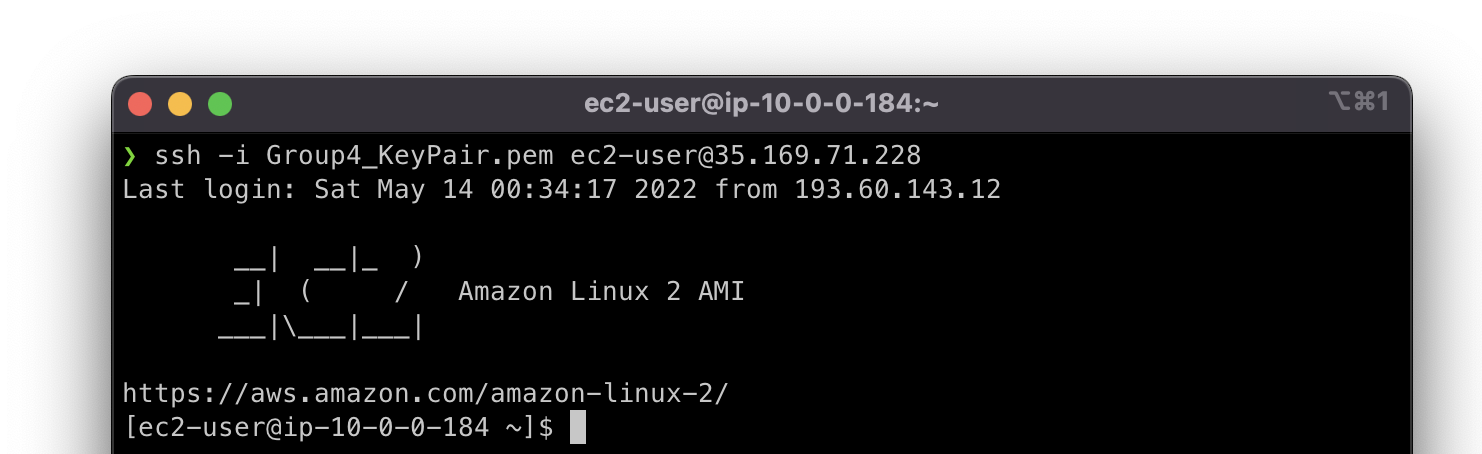
\includegraphics[width=\textwidth]{resources/ec2/ec2-logged-in}
    \caption{Logging into EC2 instance.}
    \label{fig:ec2-logged-in}
\end{figure}

The logged in EC2 instance can be seen in Figure~\ref{fig:ec2-logged-in}.

\clearpage
\section{Package Setup}\label{sec:web-app-setup}

The web app is stored on GitHub, and the AMI does not come with GitHub by default.
Git is subsequently installed via \mintinline{zsh}|yum install git|.

\begin{figure}[!htbp]
    \centering
    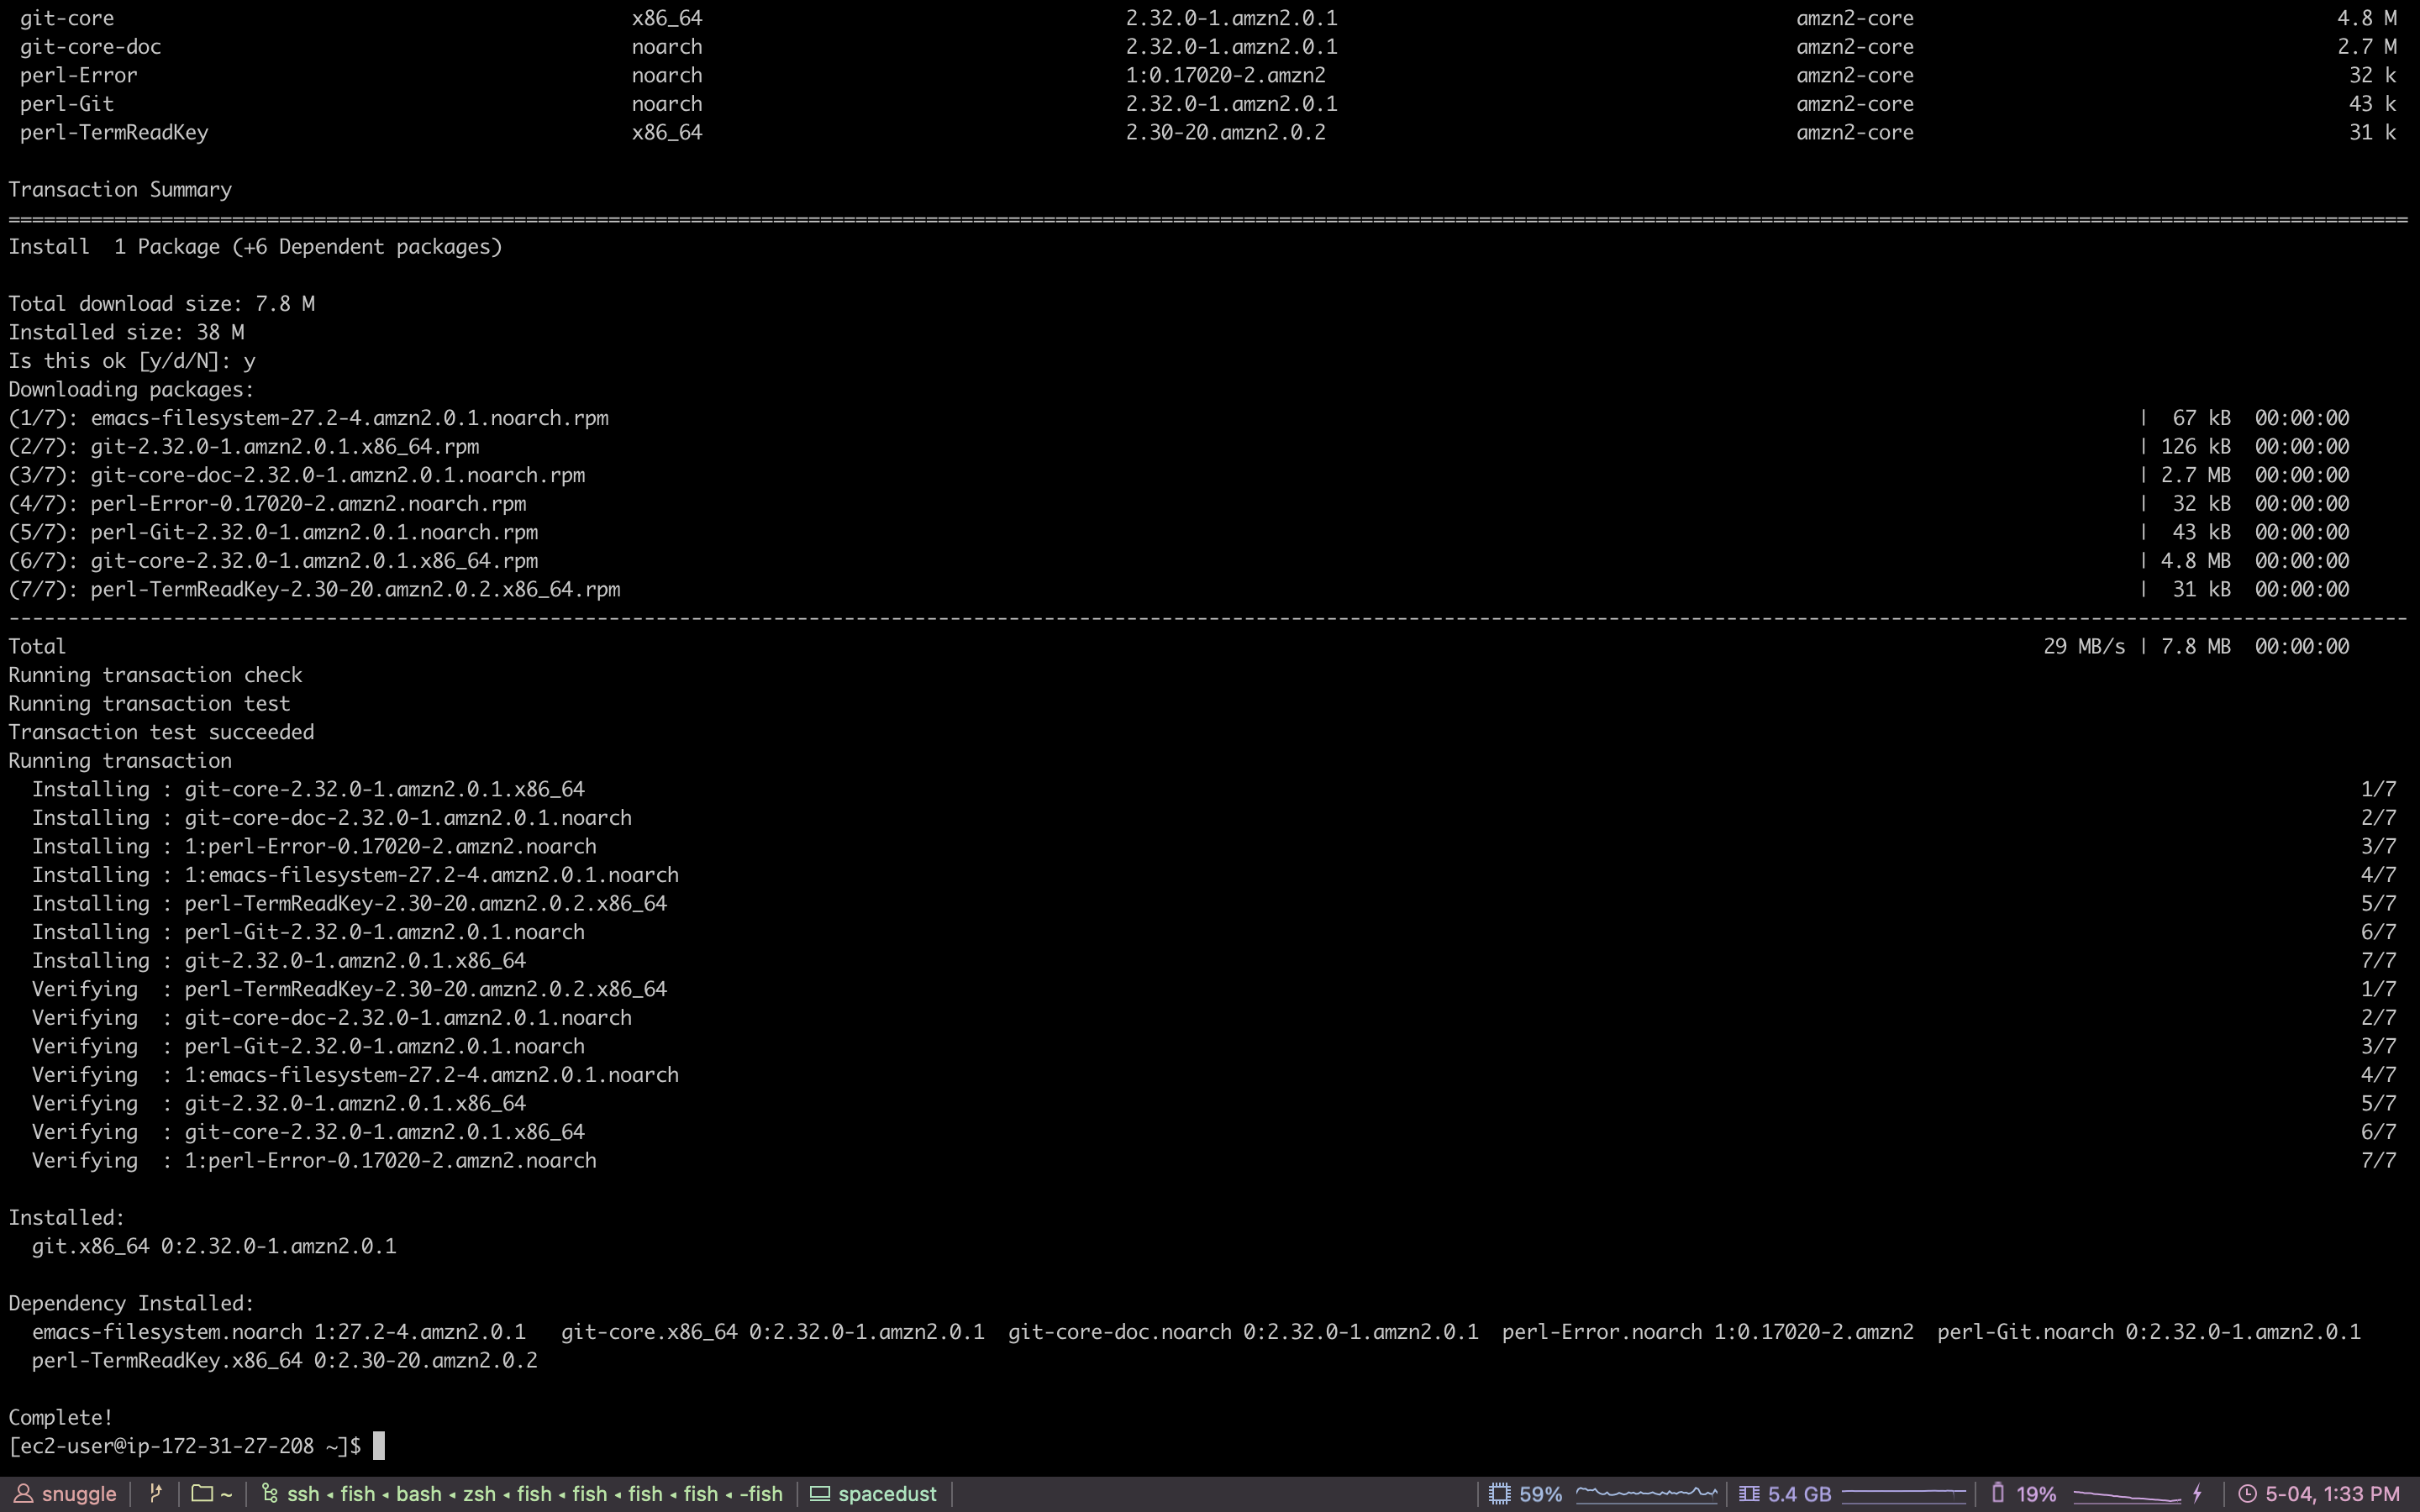
\includegraphics[width=140mm]{resources/ec2/installing-git}
    \caption{Installing Git.}
    \label{fig:webapp-git}
\end{figure}

The web app also requires docker, and \mintinline{zsh}|yum install docker| is executed to install Docker as a result.

\begin{figure}[!htbp]
    \centering
    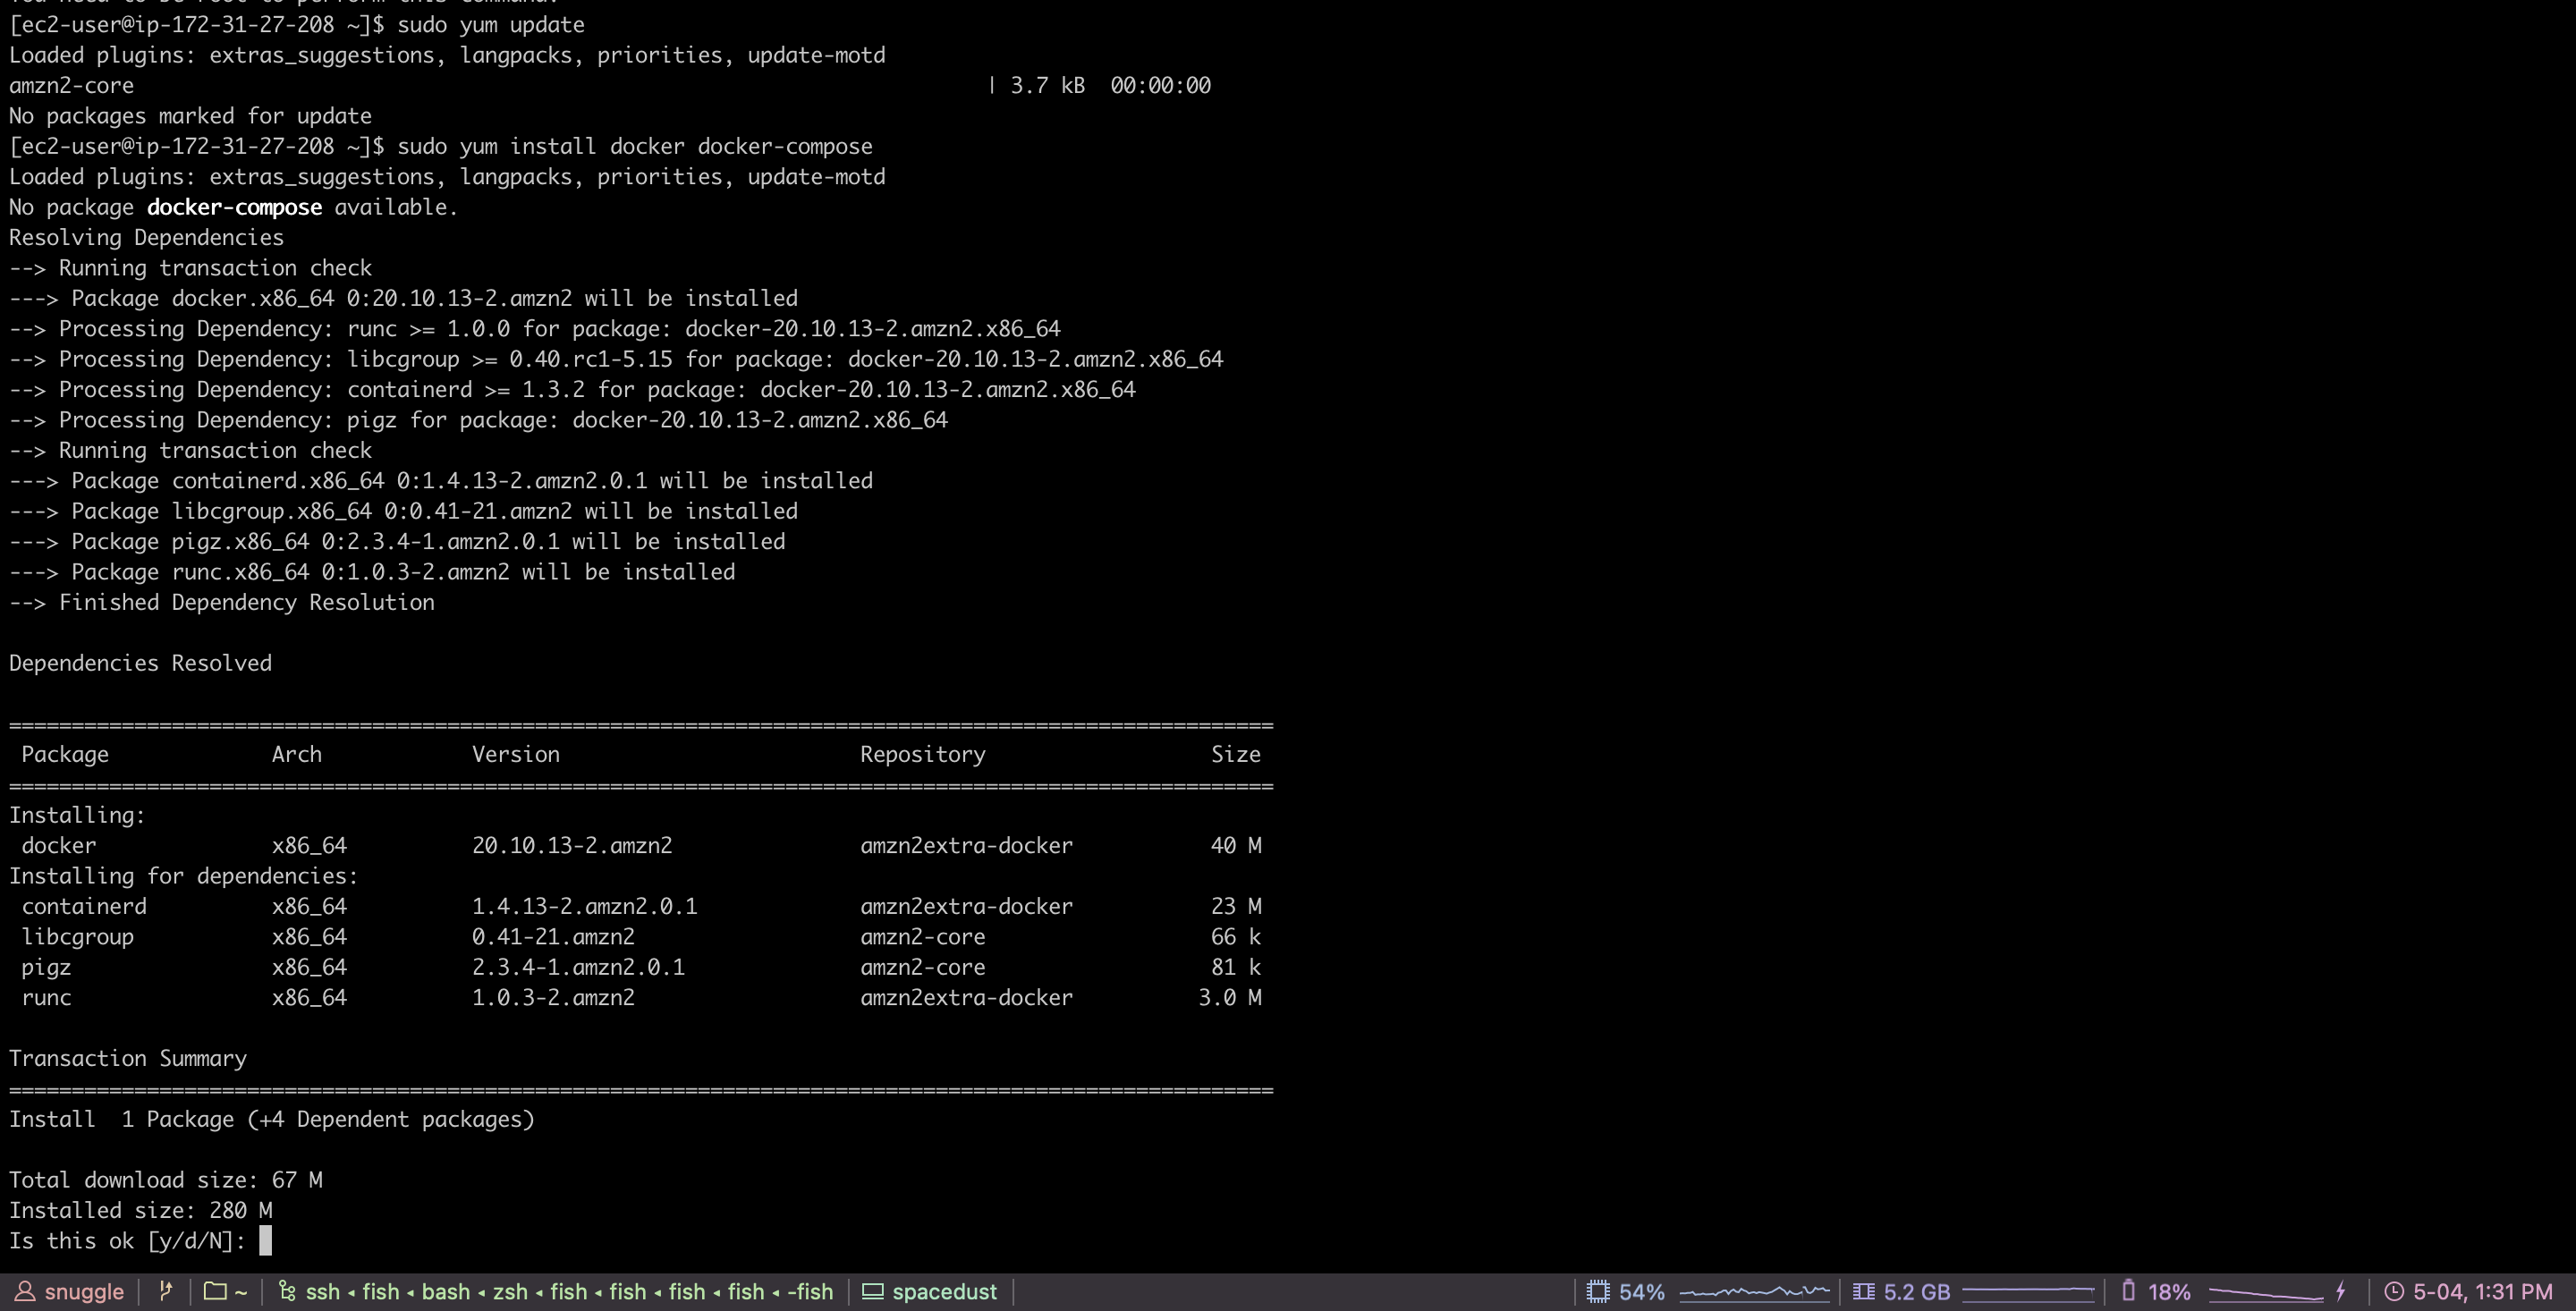
\includegraphics[width=140mm]{resources/ec2/installing-docker}
    \caption{Installing Docker.}
    \label{fig:webapp-docker}
\end{figure}

\clearpage
\section{Web App Setup}\label{sec:web-app-setup2}

The web app is firstly cloned from its repository via the \mintinline{zsh}|git clone| command, and a new
\mintinline{zsh}|digital-ink| folder is made to store the contents.

\begin{figure}[!htbp]
    \centering
    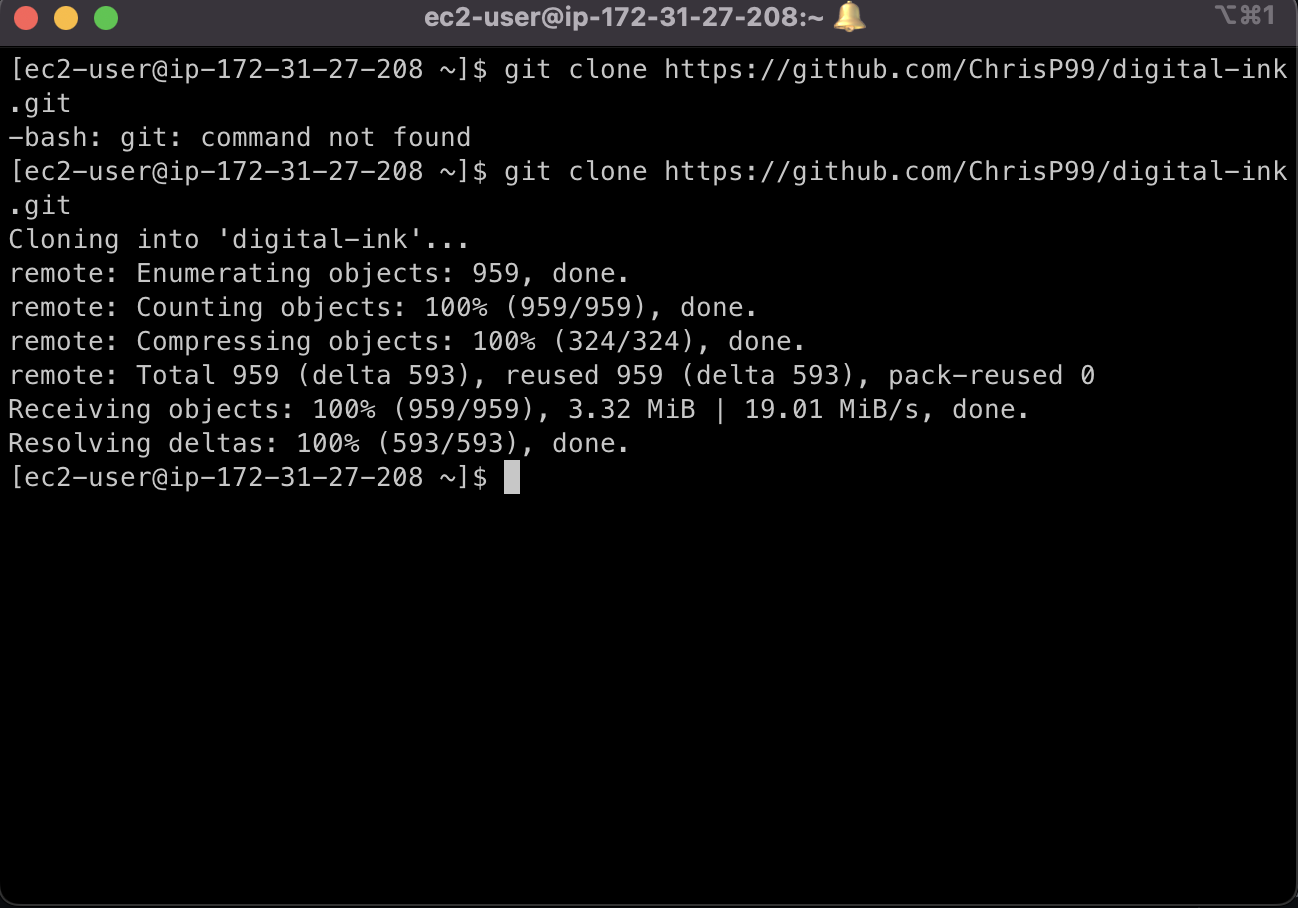
\includegraphics[width=125mm]{resources/ec2/webapp-clone}
    \caption{Cloning the web app from Github.}
    \label{fig:webapp-clone}
\end{figure}

The \mintinline{zsh}|cd| command is used to move into the \mintinline{zsh}|digital-ink| folder, and the web app is
subsequently launched through the \mintinline{docker}|docker-compose up -d| to launch the web app as a detached Docker
container.
Relevant containers that are required to be downloaded from the \mintinline{docker}|dockerfile| are then pulled.

\begin{figure}[!htbp]
    \centering
    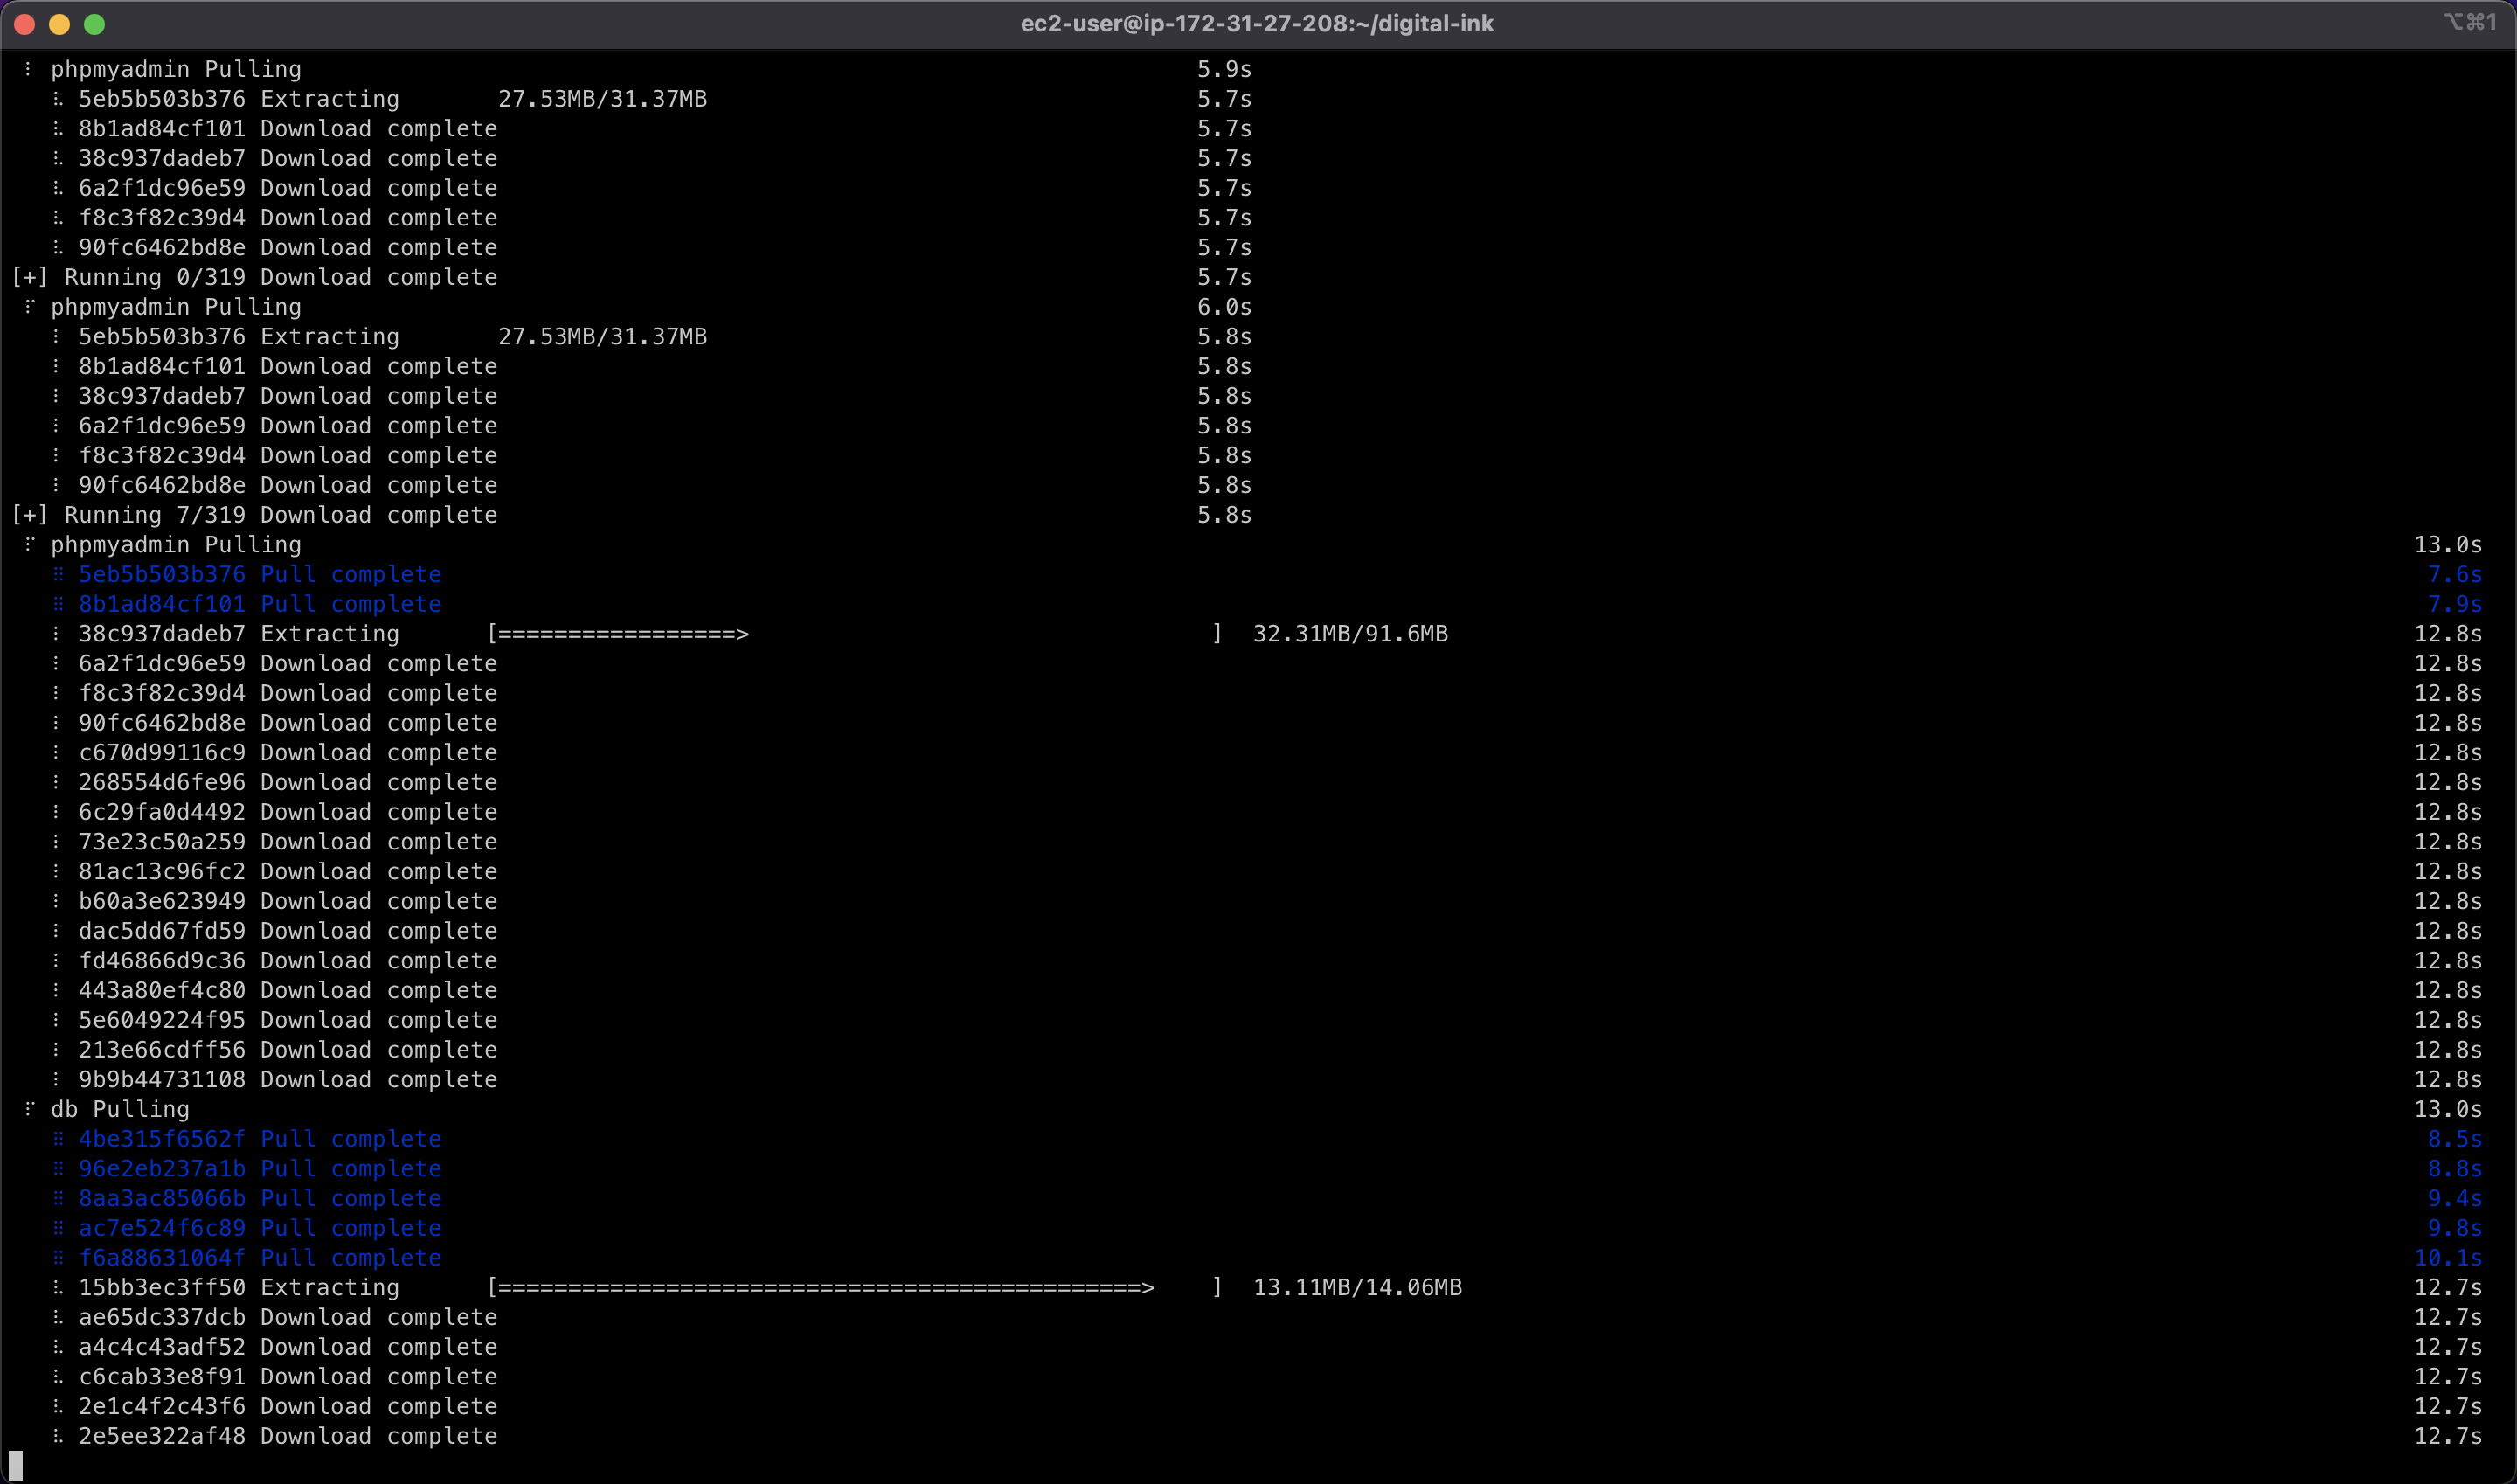
\includegraphics[width=125mm]{resources/ec2/docker-compose}
    \caption{Containers required for the web app being pulled from Docker Hub.}
    \label{fig:webapp-docker-compose}
\end{figure}

The result of this command launches 3 containers:

\begin{enumerate}
    \item \mintinline{docker}|digital-ink|: An instance of the web app which uses a custom Laravel container.
    \item \mintinline{docker}|mysql|: An instance of a local database made in MySQL\@.
    \item \mintinline{docker}|phpmyadmin|: A way to locally manage the database through a UI\@.
\end{enumerate}

\clearpage
At the minute, the web app is live through the \mintinline{docker}|digital-ink| container, and is using a local version
of MySQL as a database, stored within the \mintinline{docker}|mysql|Docker container.
The database has no tables, but can be populated through the use of Laravel.
The container is firstly accessed through \mintinline{docker}|docker exec app bash|, and the database is populated with
tables with \mintinline{zsh}|php artisan migrate|.
This then generates tables to store users and their stories.

\begin{figure}[!htbp]
    \centering
    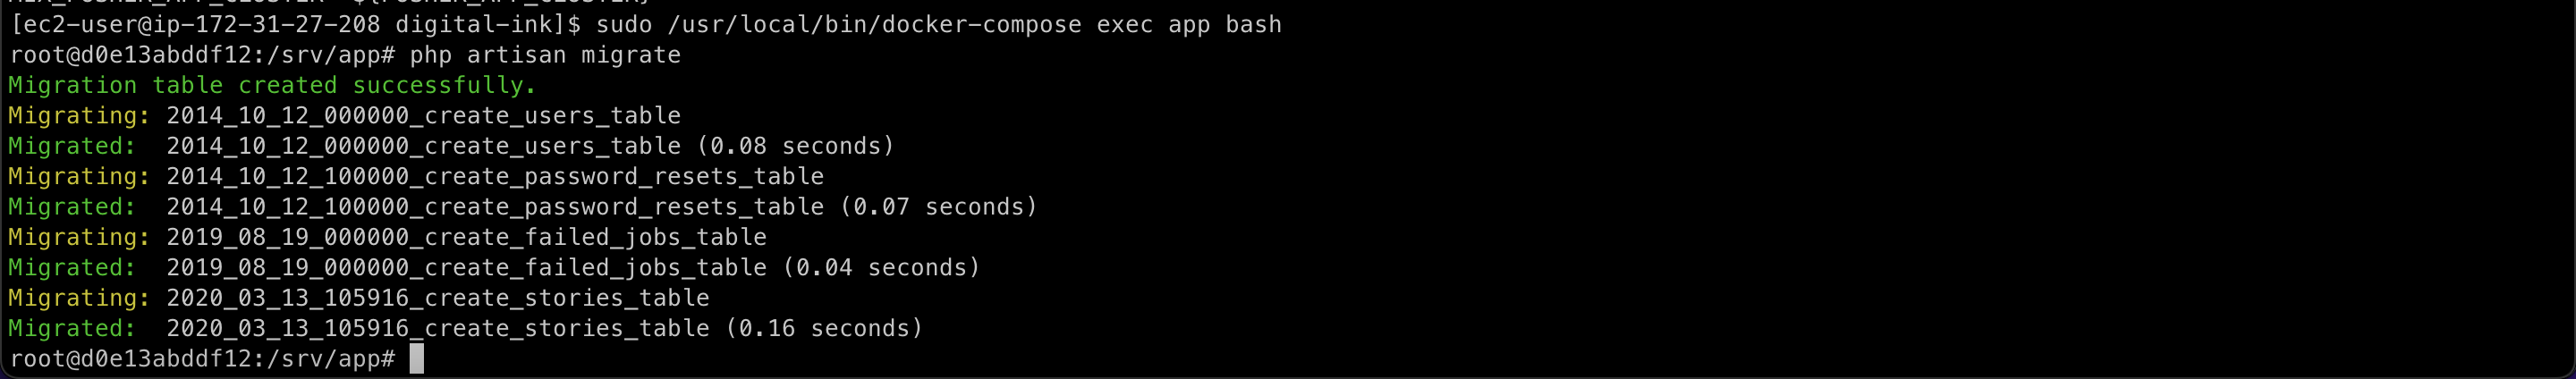
\includegraphics[width=\textwidth]{resources/ec2/php-artisan-migrate}
    \caption{Creation of tables through \mintinline{zsh}|php artisan migrate| command.}
    \label{fig:php-artisan-migrate}
\end{figure}

The subsequent output of this command can be found in Figure~\ref{fig:php-artisan-migrate}.
When the website is accessed at the public IPv4 address at \hyperlink{http://ec2-52-45-13-111.compute-1.amazonaws.com/},
Digital Ink will now be shown.

\begin{figure}[!htbp]
    \centering
    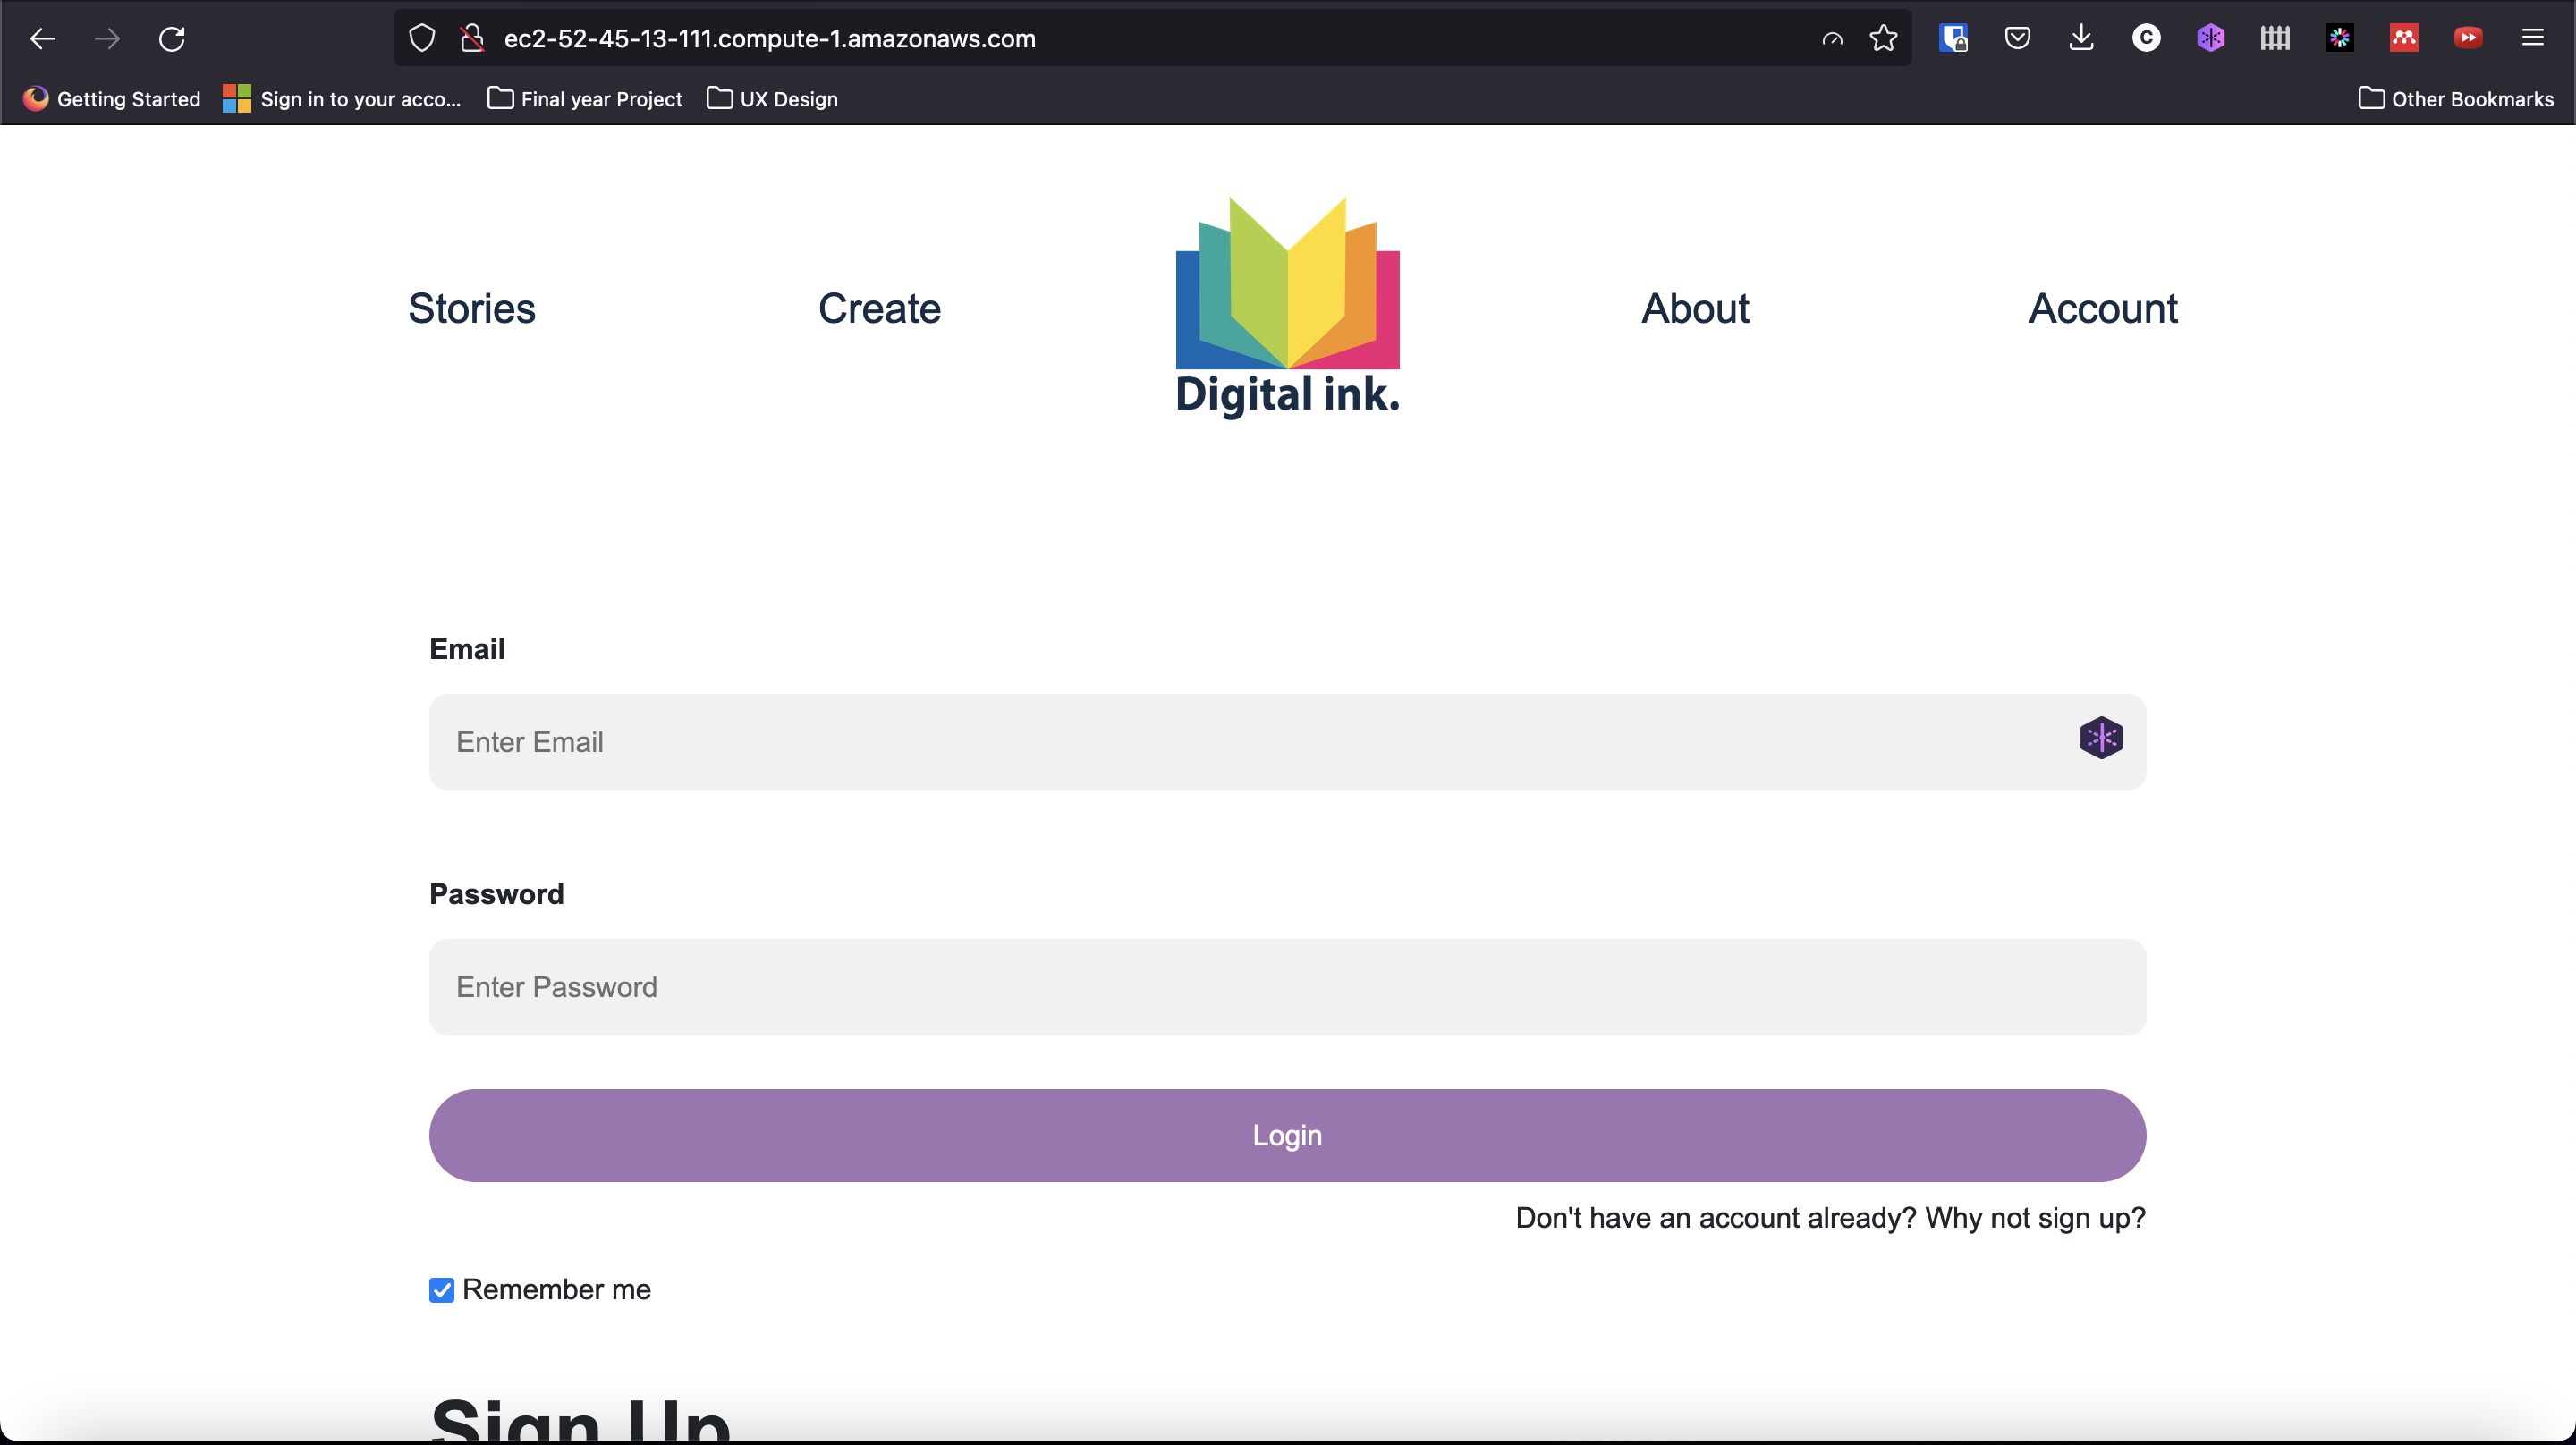
\includegraphics[width=\textwidth]{resources/ec2/digital-ink-ec2}
    \caption{Digital Ink shown when accessed through the IPv4 address. }
    \label{fig:digital-ink-ec2}
\end{figure}
